\chapter{实机调试部署技巧}
\label{chap:deployment}

\begin{introduction}
  \item 学习目标：首次用 SSH 登录目标机，在专用目录同步并试跑确定版本，记录日志与退出状态。按需练习远程桌面、网络、进程管理与 KVM。
  \item 建议学时：首次约半天，完成 SSH、试跑与日志核验。全章约 2--3 天；真实设备与长时间运行按队内计划另行验收。
  \item 本卷边界：以 Ubuntu 22.04 机载电脑与常见桌面客户端为例，讲部署和维护基本功；相机、CUDA、ROS 2 及控制链路见卷二、卷三。工具资料按 2026 年 10 月 31 日核对，软件界面和硬件型号应以实际版本为准。
\end{introduction}

\begingroup
\setlength{\emergencystretch}{3em}
\clubpenalty=10000
\widowpenalty=10000

卷零用断点回答“程序在哪一步偏离预期”。到了机载电脑，还要问“同一版本到了另一台机器，运行条件哪里变了”。现在带上前面练过的终端、Git 和 CMake 操作，先走完第~\ref{sec:deploy-physical}--\ref{sec:deploy-delivery}~节。练习需要一台 Ubuntu 目标机，以及能从笔记本到达的地址。两台机器先放在可以互通的网络中。没有可用的局域网时，先查第~\ref{sec:deploy-wired}~节。

\section{代码走出自己的电脑}
\label{sec:deploy-physical}

前面几章里，你已经能从确定的源码版本构建并运行程序。接下来，学长把机器人推过来：“放到车上跑一下吧。”这时候你才发现，\textbf{在自己的电脑上能运行，只是交付的起点}。机器人真正使用的是机载电脑（onboard computer）：程序要在它的处理器和系统上运行，读取它的相机与串口，并在重新上电后按预期工作。你电脑上的文件夹需要先同步到车上，x86 电脑编译的程序也不能直接拿给 ARM 板运行。

我们把准备目标环境、传送代码与配置、在目标机构建或安装、启动并核验结果这一过程称为\textbf{部署（deployment）}。本章先解决一个最实际的问题：怎样操作机载电脑？等连接稳定了，再讨论如何把程序放上去、让它持续运行，并在故障时找回控制权。

\subsubsection{便携屏和键鼠：最直接的入口}

最传统的办法，是给机载电脑接上一块便携显示器，再插 USB 键盘与鼠标。图~\ref{fig:deploy-monitor} 是一块带 HDMI 输入的小屏幕；对机载电脑来说，它就是普通外接显示器。你可以看到开机画面、登录桌面，像操作自己的电脑一样打开终端，网络还没配好时尤其有用。

\begin{figure}[htbp]
  \centering
  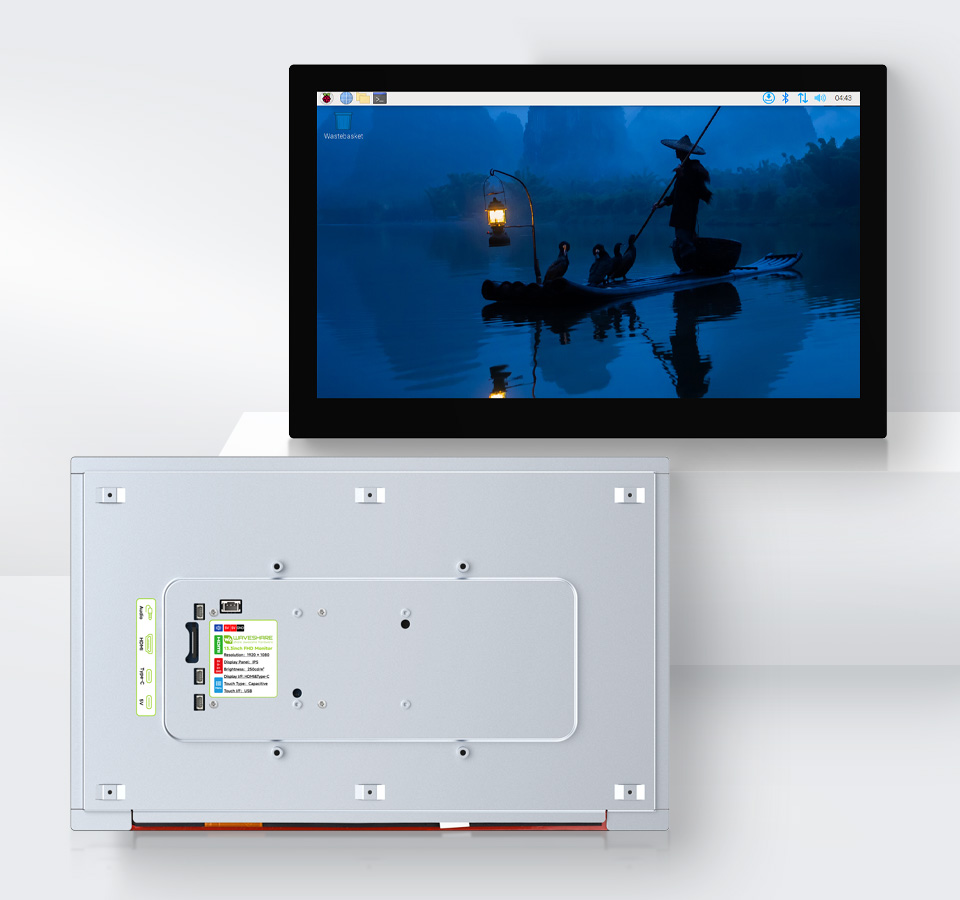
\includegraphics[width=0.58\textwidth]{deployment/portable-monitor.jpg}
  \caption{便携 HDMI 显示器的正反面。先确认视频输入与供电接口，再准备键鼠；图源：Waveshare 官方产品页。}
  \label{fig:deploy-monitor}
\end{figure}

不过，机器人通常不在桌上。你可能一边蹲在地上扶屏幕，一边伸手够键盘，旁边还拖着供电线和视频线；换个位置调车，整套“移动办公桌”又得搬一次。便携屏非常适合首次装机和故障救援，日常开发则可以让自己的笔记本承担键盘与屏幕，把终端或桌面通过连接传回来。接下来的 SSH 和远程桌面，就是为了让你少蹲一会儿。

\begin{example}[首次接入机载电脑]
前提是机载电脑已有可启动的系统，机器人处于队内确认的安全调试状态，不会因为程序误启动产生运动。一定记得注意安全，小心机器人突然甩头把屏幕键盘全部扯到地上，到时候抱着碎掉的便携屏流泪。
先核对电脑的视频\emph{输出}接口与显示器的\emph{输入}接口：HDMI 对 HDMI；只有 DP 输出时，使用方向正确的 DP 转 HDMI 适配器。按显示器铭牌准备电源，再接视频线，最后把有线键鼠插到机载电脑的 USB 口。USB-C 的外形不保证支持视频输出，也不保证能为屏幕供电，应查看两端说明书。

开机后在屏幕上选择对应输入源，确认能看到启动或登录画面。进入桌面后打开终端，运行下面两条只读命令，记录用户名与主机名；后文以用户 \texttt{rm}、主机名 \texttt{rm-robot} 为例，实际使用时换成自己的。
\begin{tbash}
whoami
hostname
\end{tbash}
如果屏幕显示“无信号”，先检查输入源、线材方向与供电，再看主机是否实际启动；此时还没进入 SSH，修改网络配置通常帮不上忙。
\end{example}

\begin{exercise}\label{ex:deploy-physical}
给队内一台机载电脑画出便携屏、屏幕电源与 USB 键鼠的接线图，标明输入和输出方向。接入后记录实际用户名、主机名以及视频接口；没有设备时先按型号手册完成接线方案，现场验证留到本章验收。
\end{exercise}

教材选图用于认识便携屏的外观，大家自行购买合适的便携屏。

\section{先把终端搬过来：SSH}
\label{sec:deploy-ssh}

便携屏能让你看到机器人上的桌面，但如果只是改参数、编译、看日志，每次搬一套外设实在有点累。安全外壳协议（Secure Shell，SSH）可以让笔记本打开机载电脑的终端：你在自己的键盘上输入，命令却在机器人上执行，结果再传回来。普通 SSH 登录只传终端数据，通常很适合远程开发。

这里先假定两台电脑已接入同一台路由器，机器人当前地址为 \texttt{192.168.50.20}，普通用户名为 \texttt{rm}。这两个值都要换成自己的；如何找到地址、用主机名代替地址以及没有路由器时怎么办，稍后在第~\ref{sec:deploy-lan}、\ref{sec:deploy-wired}~节动手。\textbf{能上网不代表两台设备之间能互通}，访客网络可能禁止客户端相互访问。

\subsubsection{装在谁上面，命令又在哪边执行}

SSH 分为客户端与服务端：笔记本运行客户端发起连接，机载电脑运行服务端接收连接。Ubuntu 上 \texttt{openssh-client} 提供前者，\texttt{openssh-server} 提供后者。Windows 10/11 通常可在 PowerShell 或终端使用 \texttt{ssh}；若找不到命令，在“可选功能”安装 OpenSSH 客户端。机载电脑装的是 Ubuntu Server 还是 Desktop，不影响使用 SSH。

\begin{example}[从笔记本进入机载电脑]
先借助便携屏，在\textbf{机器人本机终端}安装并核对服务：
\begin{tbash}
sudo apt update
sudo apt install openssh-server
sudo systemctl enable --now ssh
systemctl is-active ssh
hostname
whoami
ip -br address
sudo ssh-keygen -lf /etc/ssh/ssh_host_ed25519_key.pub
\end{tbash}
\texttt{is-active} 应输出 \texttt{active}。记下实际用户名、当前接口的 IPv4 地址，以及最后一行的 \texttt{SHA256:...} 主机指纹。若机载电脑启用了防火墙，只对调试网络放行 SSH 端口。

然后在\textbf{笔记本终端}执行，基本形式是 \texttt{ssh 用户名@地址}：
\begin{tbash}
ssh rm@192.168.50.20
hostname
whoami
pwd
exit
\end{tbash}
第一次连接会问是否信任主机密钥。把显示的指纹与刚才在机器人本机看到的指纹核对，一致再输入 \texttt{yes}，然后输入机器人上 \texttt{rm} 用户的密码；输入密码时没有星号回显是正常现象。连接后，\texttt{hostname} 应是机器人而非笔记本的名字，\texttt{pwd} 通常是远端家目录。\texttt{exit} 退出远端终端，回到笔记本。
\end{example}

如果提示 \texttt{Connection timed out}，先查地址、链路、客户端隔离与防火墙；\texttt{Connection refused} 通常表示目标拒绝该端口连接，应检查 SSH 服务和端口；\texttt{Permission denied} 则优先核对用户名、密码或密钥。用 \texttt{ssh -v rm@地址} 查看连接过程。终端提示符可自定义，容易看花眼时，主动运行 \texttt{hostname} 与 \texttt{pwd} 确认操作对象。

\begin{note}
主机密钥验证的是“你连到哪台机器”。如果以前连接过，后来出现 \texttt{REMOTE HOST IDENTIFICATION HAS CHANGED}，先核对是否重装系统、地址被另一台机器占用或连接目标错误；确认新指纹后再按文档更新记录。不要养成禁用主机密钥检查的习惯。改 SSH 配置前也应保留当前连接与本地救援入口，先运行 \texttt{sudo sshd -t} 检查配置。
\end{note}

\subsubsection{密钥和连接别名：少输一点，也更好管理}

用户密钥回答“你是谁”，与刚才用于核验服务器身份的主机密钥职责不同。私钥留在笔记本，公钥可以交给机器人；私钥密码用于保护本地私钥，也不等于机器人登录密码。下面以 Ubuntu 笔记本为例；Windows 客户端也可生成密钥，分发公钥的方法见 OpenSSH 文档。

\begin{example}[给自己的调试连接建档]
在笔记本上生成专用密钥；若该名字已存在，选新名字，不覆盖旧密钥。按提示设置私钥密码：
\begin{tbash}
ssh-keygen -t ed25519 -f ~/.ssh/id_ed25519_rm -C "rm-debug-laptop"
ssh-copy-id -i ~/.ssh/id_ed25519_rm.pub rm@192.168.50.20
ssh -i ~/.ssh/id_ed25519_rm rm@192.168.50.20
\end{tbash}
确认可登录后，退出连接，把下面一段加入\textbf{笔记本}已有的 \path{~/.ssh/config}，不要覆盖其他配置：
\begin{tbash}
Host rm-robot
    HostName 192.168.50.20
    User rm
    IdentityFile ~/.ssh/id_ed25519_rm
    IdentitiesOnly yes
    ServerAliveInterval 15
    ServerAliveCountMax 3
\end{tbash}
之后运行 \texttt{ssh rm-robot} 即可。\texttt{Host} 是本机别名，\texttt{HostName} 指定实际目标。以后可将目标改为 \path{rm-robot.local} 或 Tailscale 名称。\texttt{IdentityFile} 指明使用哪份私钥；保活参数帮助发现连接中断，不会自动重启远端程序。用 \texttt{ssh -G rm-robot} 可展开当前实际采用的客户端配置。
\end{example}

不要把私钥提交到 Git，也不要让全队共用一份个人私钥。每人使用自己的密钥，队员离队或笔记本丢失时，你就可以在机载电脑上单独撤销对应的公钥。公钥登录先在另一个终端验证成功，再考虑是否调整密码登录策略，避免把自己锁在门外。

\begin{exercise}\label{ex:deploy-ssh}
使用自己的两台设备完成一次 SSH 登录，记录客户端与服务端的主机名、用户名和主机指纹核验方式。再添加一个连接别名，以密钥登录，说明公钥、私钥、主机密钥分别保存在哪里、负责验证谁。只有一台机器时可先在虚拟机练习，并明确标注不是实机验收。
\end{exercise}

\begin{conclusion}
SSH 让你远程使用终端；它需要网络可达、远端服务启动及身份验证成功。IP 地址或可解析的名字负责找机器，主机指纹负责确认机器，用户名与用户密钥负责登录。断开 SSH 后程序是否继续运行，还取决于会话与进程的启动方式，见第~\ref{sec:deploy-ops}~节。
\end{conclusion}

安装与服务检查可查 \href{https://ubuntu.com/server/docs/how-to/security/openssh-server/}{Ubuntu OpenSSH 指南}；密钥和客户端配置参数分别见 \href{https://man.openbsd.org/ssh-keygen}{ssh-keygen 手册}、\href{https://man.openbsd.org/ssh_config}{ssh\_config 手册}。

\Needspace{10\baselineskip}
\subsubsection{用 SSH 显示远程窗口（选读）}
\label{sec:deploy-x11-forwarding}

有时只想打开机载电脑上的一个配置工具。若程序支持 \textbf{X11}，可以让它在机载电脑上运行，通过 SSH 把窗口显示在笔记本上。程序仍读取机载电脑上的文件，也仍使用那台电脑的资源。要接管机载电脑已有的整个桌面，见第~\ref{sec:deploy-desktop}~节。

X11 和 \textbf{Wayland} 都是 Linux 图形程序与显示系统之间的协议。使用 X11 时，程序通过 X 服务器显示窗口和接收输入，SSH 可以转发这条 X11 连接。使用 Wayland 时，原生程序连接到负责合成窗口和分发输入的 Wayland 合成器。\textbf{Xwayland} 是在 Wayland 会话中为 X11 程序提供兼容性的 X 服务器。

\Needspace{10\baselineskip}
\begin{example}[让机载电脑上的时钟显示在笔记本]
先确认普通 SSH 已能登录。在\textbf{机载电脑}上安装授权工具和测试程序，然后检查 SSH 服务端的配置。
\begin{tbash}
sudo apt install xauth x11-apps
sudo sshd -T | grep -E '^x11(forwarding|uselocalhost) '
\end{tbash}
预期看到 \texttt{x11forwarding yes} 和 \texttt{x11uselocalhost yes}。如果服务端尚未允许转发，在机载电脑上编辑 \path{/etc/ssh/sshd_config} 或其中引用的配置文件，启用 \texttt{X11Forwarding yes}，保留 \texttt{X11UseLocalhost yes}。保持现有 SSH 连接，先用 \texttt{sudo sshd -t} 检查配置，确认通过后在 Ubuntu 上用 \texttt{sudo systemctl reload ssh} 重载。

\Needspace{9\baselineskip}
在\textbf{笔记本的图形终端}打开一条新连接。Ubuntu 笔记本可用 \texttt{sudo apt install xauth} 安装本地授权工具。第一行在笔记本执行，其余三行在连上后的远端终端执行。
\begin{tbash}
ssh -X rm-robot
hostname
echo "$DISPLAY"
xclock
\end{tbash}
主机名应是机载电脑的名称，\texttt{DISPLAY} 通常类似 \texttt{localhost:10.0}，这个地址由 SSH 分配，保留它即可。时钟窗口应出现在笔记本上。关闭窗口后，远端终端会回到提示符。机载电脑可以只运行命令行系统，只需具备 SSH 服务、授权工具和要打开的程序。
\end{example}

没有窗口时，先按下文检查笔记本能否打开本地 X11 显示，再用 \texttt{ssh -v -X rm-robot} 检查转发请求是否被接受。远端的 \texttt{DISPLAY} 为空时，优先核对服务端配置和两端的 \texttt{xauth}。\texttt{-X} 使用受限制的转发，某些程序或本地 X 服务器可能不支持。若确认问题出在这一限制，可仅对信任的主机和程序试用 \texttt{ssh -Y rm-robot}。\texttt{-Y} 会给予远端程序访问笔记本 X11 会话的较大权限。详见 \href{https://man.openbsd.org/ssh#X11_FORWARDING}{OpenSSH 的 X11 转发说明}。

\Needspace{7\baselineskip}
\textbf{笔记本平时用 Wayland 怎么办}

先从\textbf{笔记本的桌面}打开一个新的普通用户终端。这里查的是笔记本的显示环境，所以在发起 SSH 之前执行下面的命令。
\begin{tbash}
printf 'XDG_SESSION_TYPE=%s\nDISPLAY=%s\n' "$XDG_SESSION_TYPE" "$DISPLAY"
command -v Xwayland
\end{tbash}
\texttt{XDG\_SESSION\_TYPE} 显示 \texttt{wayland} 时，\texttt{command -v Xwayland} 可检查是否找得到 Xwayland 程序，常见路径是 \path{/usr/bin/Xwayland}。有这个路径只说明找得到程序。\texttt{DISPLAY} 若有值，例如 \texttt{:0}，再实际连一次 X 显示。Ubuntu 上缺少 \texttt{xprop} 时，可在笔记本上用 \texttt{sudo apt install x11-utils} 安装。
\begin{tbash}
xprop -root >/dev/null && echo "X11 OK"
\end{tbash}

\begin{itemize}
  \item \textbf{显示 \texttt{X11 OK}。}笔记本当前终端能连接 X 服务器，可以保留当前会话，用上面的 \texttt{ssh -X} 转发。机载电脑上的程序要支持 X11。有多个图形后端时，可在远端启动命令前加 \texttt{GDK\_BACKEND=x11}（GTK）或 \texttt{QT\_QPA\_PLATFORM=xcb}（Qt），前提是已安装相应后端。
  \item \textbf{\texttt{DISPLAY} 为空，或提示 \texttt{unable to open display}。}先回到笔记本桌面，用当前登录用户打开新终端复查。若 Ubuntu 22.04 的 GNOME 会话缺少 Xwayland，在笔记本上运行 \texttt{sudo apt install xwayland}，退出桌面并重新登录，再跑一次检查。若已经安装，按所用桌面的说明确认 Xwayland 支持已启用。显示地址由桌面会话提供，手动填一个 \texttt{:0} 无法启动 Xwayland。
  \item \textbf{仍没有可用的 X11 显示。}如果程序支持原生 Wayland，可以改用下面的 \texttt{waypipe}。如果程序只支持 X11，可在笔记本切换到可用的 Xorg 会话再检查。Ubuntu 22.04 的 GNOME 登录页可在选中用户名后，通过齿轮选择 \href{https://documentation.ubuntu.com/release-notes/22.04/}{Ubuntu on Xorg}。也可按第~\ref{sec:deploy-desktop}~节连接机载电脑的远程桌面，在其支持 X11 的图形会话里启动程序。
\end{itemize}

\Needspace{6\baselineskip}
原生 Wayland 窗口可以用 \texttt{waypipe} 经 SSH 转发到笔记本的 Wayland 会话。两端都要安装 \texttt{waypipe}，并允许 SSH 转发 Unix 套接字。在 Ubuntu 22.04 可从 \texttt{universe} 软件源安装 \texttt{waypipe}。在机载电脑安装 \texttt{gtk-4-examples} 后，从笔记本的 Wayland 图形终端运行下面的命令。
\begin{tbash}
waypipe ssh rm-robot env GDK_BACKEND=wayland gtk4-demo
\end{tbash}
窗口能出现并响应操作，才算这个程序的转发成功。两端版本、图形接口及应用依赖会影响兼容性。若要看相机的实时画面或跑依赖 GPU 的图形工具，先用真实数据测延迟和帧率，再选入口。参见 \href{https://wayland.freedesktop.org/docs/book/Xwayland.html}{Wayland 的 Xwayland 说明}和 \href{https://manpages.ubuntu.com/manpages/jammy/man1/waypipe.1.html}{Ubuntu 22.04 的 waypipe 手册}。

\begin{exercise}\label{ex:deploy-x11}
记录笔记本的会话类型、本地 \texttt{DISPLAY} 和 \texttt{xprop} 的检查结果。若本地 X11 显示可用，连接 SSH 后记录远端主机名和 SSH 分配的 \texttt{DISPLAY}，打开时钟并指出程序和窗口分别在哪台电脑上。若本地检查失败，说明你会先检查哪一项，以及仅支持 X11 和支持原生 Wayland 的程序分别可走哪条路线。
\end{exercise}

\subsubsection{远程编辑：VS Code Remote -- SSH（选读）}
如果已经按卷零第 1 章在本机用过 VS Code，这里可以沿用熟悉的编辑界面，把打开的工程换成机器人上的目录。


SSH 不要求你只能用终端编辑器。第 1 章用过的 VS Code 可安装 Microsoft 的 \texttt{Remote - SSH} 扩展，在笔记本显示界面，在机载电脑读写工程、运行终端与调试器。这属于远程开发：它不会直接把机器人的整个桌面搬过来，也不会自动把所有本地文件同步过去。

\begin{example}[确认编辑与编译发生在哪台电脑]
先在普通终端验证 \texttt{ssh rm-robot} 成功，再在\textbf{笔记本}的 VS Code 扩展页安装 \texttt{Remote - SSH}。打开命令面板，选择 \texttt{Remote-SSH: Connect to Host...}，选择配置好的 \texttt{rm-robot}。首次连接会在远端安装 VS Code Server，需要可用下载通路及满足扩展要求的系统与资源；离线场地应提前准备。

连接后检查状态栏显示远程主机，再用 \texttt{File > Open Folder} 打开\textbf{远端}工程目录。在新建的集成终端运行 \texttt{hostname}、\texttt{pwd} 和 \texttt{uname -m}，应看到机器人的主机名、目录和体系结构。打开一个练习文本，加入一行并保存；在独立 SSH 终端用 \texttt{cat} 读取相同的远端路径，确认修改落在远端。C++、CMake 等开发扩展按提示安装到远端，编译器与依赖也需要在远端准备。
\end{example}

\begin{exercise}\label{ex:deploy-remote-editor}
用远程窗口打开一个练习工程，从远端集成终端构建或运行本章心跳示例。把 \texttt{hostname} 与当前路径记入日志，再指出本地窗口与远程窗口各修改哪个文件系统。若安装失败，保留扩展日志，区分 SSH 连接失败与远端 Server 安装失败。
\end{exercise}

新版本对远端 Linux 的库版本、架构与下载条件可能有不同要求，安装前核对 \href{https://code.visualstudio.com/docs/remote/ssh}{Remote -- SSH 官方教程}和其中的系统要求；这也适用于资源有限的 ARM 机载电脑。

\section{连上以后，把哪一版程序送上车}
\label{sec:deploy-delivery}

SSH 登录成功以后，就可以开始部署（Deployment）：把明确版本的代码、依赖、模型和配置放到目标机器，在那里构建或安装，再核对程序是否按约定运行。\textbf{连得上只是维护入口可用，不是视觉系统已经能上场。}

先记录三件事：要部署哪个 Git 提交，目标平台和依赖是什么，如何判断这次部署成功。笔记本常见的 \texttt{x86\_64} 与机载 ARM 的 \texttt{aarch64} 不是同一架构；把前者的可执行文件复制过去，可能直接得到 \texttt{Exec format error}。动态库、GPU 驱动、CUDA、相机 SDK、模型推理后端也各有版本约束。初学时优先在目标机用源码重新构建，交叉编译及板卡工具链留给专项工程。

\subsubsection{用独立目录试跑，再保留能回去的版本}

同步文件可用 \texttt{scp}，基本形式是 \texttt{scp 本地文件 用户@地址:远端目录/}；复制目录加 \texttt{-r}。文件较多、会反复部署时可用 \texttt{rsync}，它能比较并传送变化。通过 SSH 传输时，基本形式为 \texttt{rsync [选项] 源目录/ 主机:目标目录/}。\texttt{-a} 保留常见文件属性，\texttt{-v} 显示过程，\texttt{-n} 只预览。两端都需要安装 \texttt{rsync}；下面使用第~\ref{sec:deploy-ssh}~节的 SSH 别名。

\begin{example}[先同步安全的小项目，再处理真实视觉工程]
先在\textbf{笔记本}进入本卷目录，确认有 \path{examples/deployment-demo/}。通过 SSH 新建目标机上的练习目录。若提示同名目录已经存在，先换一个目录名，后续命令也一起换，避免覆盖上一次练习。

\begin{tbash}
ssh rm-robot 'mkdir ~/rm-deploy-demo'
\end{tbash}

如果两端都有 \texttt{rsync}，在笔记本上先预览，再传输。Ubuntu 上缺少这个工具时，可用 \texttt{sudo apt install rsync} 安装。
\begin{tbash}
rsync -avn examples/deployment-demo/ rm-robot:rm-deploy-demo/
rsync -av examples/deployment-demo/ rm-robot:rm-deploy-demo/
\end{tbash}
源目录末尾的斜杠表示传输目录里的内容。使用 Windows PowerShell 等已有 \texttt{scp} 的终端时，可以逐个复制同一组文件：
\begin{tbash}
scp examples/deployment-demo/heartbeat.py rm-robot:rm-deploy-demo/
scp examples/deployment-demo/rm-heartbeat.service rm-robot:rm-deploy-demo/
scp examples/deployment-demo/README.md rm-robot:rm-deploy-demo/
\end{tbash}
传完后登录目标机，确认 \path{~/rm-deploy-demo/heartbeat.py} 存在，且 \texttt{python3 heartbeat.py --help} 在该目录下能显示帮助。
\end{example}

\subsubsection{前台试跑并核对日志}
\label{sec:deploy-first-log}

心跳程序只用 Python 标准库。它打印 PID、版本标记、工作目录和 UTC 时间戳，再按间隔输出序号。\texttt{--count} 控制次数，\texttt{--fail-after} 模拟在第几次输出后失败，便于检查能否分辨正常与异常退出。完整脚本如下：

\lstinputlisting[language=Python,numbers=left,numberstyle={\color{gray}\tiny}]{examples/deployment-demo/heartbeat.py}

\begin{example}[在 SSH 终端记录正常与异常退出]
在\textbf{目标机的 SSH 终端}运行。\texttt{> 文件 2>\&1} 将标准输出和错误都写入日志。用 \texttt{\$?} 立即记录 Python 的退出状态，再查看日志。

\begin{tbash}
cd ~/rm-deploy-demo
hostname
pwd
python3 heartbeat.py --count 3 --interval 0.2 > heartbeat-ok.log 2>&1
printf 'exit=%s\n' "$?"
tail -n 4 heartbeat-ok.log
python3 heartbeat.py --count 5 --interval 0.2 --fail-after 2 > heartbeat-fail.log 2>&1
printf 'exit=%s\n' "$?"
tail -n 4 heartbeat-fail.log
\end{tbash}

第一份日志应有三次心跳，退出状态为 0；第二份在两次心跳后记录模拟失败，退出状态为 1。两份日志开头的版本和工作目录应该一致，PID 则来自各次启动。把目标主机名、同步的版本、命令与两份日志放进交接记录。计数跑完会自行退出，持续运行的前台练习可按 Ctrl+C 停止。
\end{example}

\begin{exercise}\label{ex:deploy-first-log}
在目标机把正常试跑次数改为 4，另存一份日志。预先写下你期待的最后一条心跳和退出状态，运行后核对，并用启动信息说明程序是从哪个目录运行的。
\end{exercise}

\subsubsection{把试跑步骤用到真实 C++ 工程}

在目标机建立新的候选目录，从确定的提交取源码；在该目录单独配置、构建和安装。不要把笔记本的 \path{build/} 一起搬过去，CMake 缓存可能记录了笔记本上的编译器和绝对路径。第 3 章的构建命令仍然适用，只是这次在\textbf{机器人 SSH 终端}运行：
\begin{tbash}
uname -m
cmake -S . -B build -DCMAKE_BUILD_TYPE=Release
cmake --build build -j2
cmake --install build --prefix "$HOME/rm-candidate/install"
\end{tbash}
这里假定当前目录就是带有安装规则的候选工程，\path{~/rm-candidate/install} 是本次专用目录。\texttt{-j2} 用两个并行任务，内存紧张的板子可从 \texttt{-j1} 开始；开发机上“线程全开”的习惯搬到小板上，可能先把内存吃光。安装后还需按工程说明传入配置、模型与测试数据，从真实安装位置试跑。

版本不能只靠文件夹名字记。保存源码提交号、未提交修改状态、模型与配置的校验值，以及目标机环境；模型太大不适合直接放 Git 时，也应记录可追溯的存储位置与散列值。修改配置同样会改变行为，不能只记“源码没动”。

\begin{tbash}
git rev-parse HEAD
git status --short
sha256sum config.yaml model.onnx
uname -m
cat /etc/os-release
\end{tbash}
上面最后一组命令在\textbf{真实工程根目录}执行，文件名换成实际的配置与模型。它们不是心跳项目的文件。把输出和启动命令、测试时间、实际结果写入部署记录，便于队友复现。

\begin{exercise}\label{ex:deploy-delivery}
把心跳项目同步到另一台机器的专用目录，确认层级正确，并比较两端 \texttt{heartbeat.py} 的 SHA-256 值。再为自己的 C++ 项目写一份部署记录模板，至少包含版本、架构、依赖、配置、启动方式、验证结果和回退办法。不要把当前可用的比赛目录拿来做覆盖练习。
\end{exercise}

\begin{conclusion}
保留当前已验证版本，在独立目录试跑候选；验收通过后再按队内流程切换。回退要能恢复\textbf{程序、配置与模型的配套组合}，并重新核对启动入口。旧版本放在 Git 提交、发布目录或规范的制品存储中，不靠在源码树里不断增加 \texttt{old2\_final\_reallyfinal} 来维持记忆。
\end{conclusion}

\subsubsection{软件通过以后，还要看真实输入与连续运行}

先用固定录像或心跳程序确认部署流程，再接相机、串口与控制。检查设备权限、相机实际分辨率和帧率、输入输出时间戳、CPU/GPU 占用、内存和温度，以及掉线后的恢复。长时间测试要记录约定时长和实际结束状态；只截一张“进程还在”的图，无法证明整个期间都在正常处理数据。

\begin{example}[给一次板端试跑写清证据]
试跑前，由负责人确定机器人固定方式、允许的动作与停止入口；涉及执行器时，先与电控同学核对安全测试状态。记录候选提交、参数和输入，先跑固定回放核对输出，再在允许状态接入真实设备。试跑过程中保存启动日志、设备断连与重连日志、处理速率及延迟口径、温度和资源采样。结束后写明实际时长、是否异常退出、如何停止，以及是否恢复到当前可用版本。

没有相机或板子时，可以完成文件传输、环境核对与软件回放，把相机输入、功耗温度、真实串口与连续运行列为待验证；不能用“回放通过”替它们打勾。
\end{example}

\begin{exercise}\label{ex:deploy-acceptance}
把“机器人上能跑就行”改写成可检查的验收要求。任选一个视觉功能，分别写出文件与启动、固定输入、真实设备、约定时长运行四类证据，并指出哪两项不能由自己的笔记本回放替代。阈值由实际项目确定，不猜一组好看的数字。
\end{exercise}

文件传输选项与目录末尾斜杠的细节可查 \href{https://download.samba.org/pub/rsync/rsync.1}{rsync 官方手册}；硬件相关依赖与测试则以目标板及对应 SDK 文档为准。


\section*{按任务选读}
\phantomsection
\addcontentsline{toc}{section}{按任务选读}

首次试跑完成后，可以直接去第~\ref{sec:deploy-assessment}~节核对结果。需要看单个窗口，可回到第~\ref{sec:deploy-x11-forwarding}~节；需要操作整个桌面，就继续读远程桌面。需要换一种连接方式就查局域网、直连或 Tailscale。需要保留会话、管理服务或在系统网络不可用时救援，再查相应的运维与 KVM 小节。

\section{装好工具，先选对入口}
\label{sec:ai-desktop}

前面讲的原理可以用来选择不同厂商、不同客户端的 AI 工具。接下来，我们以 \textbf{ChatGPT 桌面版和 Codex CLI} 演示具体操作；你也可以使用已有的其他工具，按相同标准检查它能读取什么、能执行什么、怎样验证结果。先判断眼前任务需要哪种工作方式，再寻找软件中的对应入口，安装时就不会被一堆产品名绕晕。

以下软件示例的界面与命令按 \textbf{2026 年 10 月 31 日}的官方文档核对。功能会随版本、操作系统、账号方案和工作区权限变化；找不到某个入口时，先核对这些条件，再查看相应官方页面，不要照着旧教程强行寻找同一个按钮。

\subsubsection{先按任务选择工作方式，再选择客户端}

\textbf{普通聊天}适合问概念、比较思路、讨论需求，或针对一小段代码请它逐步讲解；这时你主要阅读回答，再决定下一步。需要查资料、读取实验记录、分析数据并制作报告时，可以选择支持\textbf{多步骤工具任务}的工作方式，让 AI 调用工具、读取结果后继续处理。需要进入源码工程，搜索文件、修改代码、执行命令并读取报错时，则适合具备相应工具的\textbf{代码代理（Coding Agent）}。代码代理的价值来自“查看工程—采取行动—验证结果”的循环，而不只是一次生成更长的回答。

这些工作方式没有绝对互斥的边界。同一产品可以在聊天中启用搜索、文件或代码工具，代码代理也能只讨论而不修改。判断时应查看\textbf{当前启用的工具、执行环境和权限}，不能只看产品叫“聊天”还是“代理”。在本例软件中，ChatGPT 的 \textbf{Chat} 用于对话，\textbf{Work} 用于多步骤资料与产物任务，\textbf{Codex} 提供工程开发入口；这些菜单名称并不是所有产品通用的分类。

\textbf{命令行客户端（Command Line Interface，CLI）描述的是使用入口，不是另一种模型能力。}例如 Codex CLI 是使用 Codex 的终端入口。桌面客户端适合同时看对话、文件预览、浏览器和代码差异；CLI 适合已经在终端、SSH 服务器或开发容器中工作的你。能否执行代码任务，仍取决于连接的代理、主机工具、环境、权限和资料。

\begin{center}
\begin{tabular}{p{0.23\textwidth}p{0.32\textwidth}p{0.35\textwidth}}
\toprule
通用角色与本例入口 & 适合眼前什么事 & 你应当检查什么 \\
\midrule
普通聊天，例如 ChatGPT / Chat & 解释互斥锁、比较两种接口、用小例子讲清报错 & 推理和示例是否正确，能否自己复述 \\
多步骤工具任务，例如 ChatGPT / Work & 查资料、分析实验记录、制作报告和图表 & 来源、数据口径、产物内容与版面 \\
代码代理，例如桌面版中的 Codex & 在工程中修复问题，同时查看差异与运行界面 & 修改范围、代码差异、测试和实际行为 \\
CLI 客户端，例如 Codex CLI & 在终端、SSH 或容器内使用代码代理 & 当前目录、运行主机、环境、命令和差异 \\
\bottomrule
\end{tabular}
\end{center}

\begin{example}[同一个问题，按阶段选择工作方式]
假设你的小程序偶尔卡在退出阶段。先在你使用的聊天工具中问：“用最短 C++ 例子解释条件变量为什么需要等待谓词，再让我判断一个反例。”这一步的结果应当是你能说清虚假唤醒和退出条件。在本例软件中，可以从 ChatGPT / Chat 开始。

接着，让有权访问练习副本的代码代理定位并修复，给出复现命令、预期退出方式和实际现象，要求它指出涉及的线程、锁和退出路径，并实际运行验证。在本例中可以选择桌面版的 Codex；如果工程在远程 Linux 上，也可以 SSH 到那台机器，在工程目录启动 Codex CLI。此时你检查的是工程改动，不能只收到一段“建议这样写”。切换客户端或新开聊天后，要重新确认必要结论、文件路径与复现步骤是否已提供；同一产品若能直接切换工具，也应核对当前权限和工作目录。
\end{example}

\begin{exercise}\label{ex:ai-desktop-entry}
分别为“解释引用折叠”“在板端修复 CMake 链接失败”“把三次实验的日志整理成图表”选择工作方式与合适的客户端，可以使用本例软件或已有的其他工具，并写出各自最重要的一条验收标准。说明为什么 CLI 不是另一种模型能力，为什么不能只凭产品名称判断能否操作工程。
\end{exercise}

\subsubsection{安装桌面版、CLI 与登录}

下面进入本例软件的安装与操作：\textbf{下载地址、按钮名称和 \texttt{codex} 命令只对应 ChatGPT 桌面版及 Codex CLI}。使用其他产品时，按其官方说明安装与配置，再沿用前面的任务选择和验证方法。

从\href{https://learn.chatgpt.com/docs/app}{官方桌面版指南}进入下载页，按操作系统和处理器架构选择安装包。Windows 和 macOS 用户运行官方安装程序，按照系统提示安装，然后打开 ChatGPT 并选择 \textbf{Continue to sign in}，在浏览器完成账号登录，返回应用。不要从不明网盘下载“免登录增强版”，也不要把登录令牌交给别人代为配置。

Linux 桌面版目前处于预览阶段。官方支持列表包括 Ubuntu 24.04 / 26.04 LTS、Debian 13、Fedora 43 / 44，以及完整更新的 Arch Linux，提供 x64 与 ARM64 包。\textbf{本书其他章节常用的 Ubuntu 22.04 不在这份正式支持列表内}；不方便升级时可以先使用 Codex CLI。发行版支持与限制以\href{https://learn.chatgpt.com/docs/linux/linux-app}{Linux 安装指南}为准。

\begin{example}[在受支持的 Ubuntu 上安装]
前提是 Ubuntu 24.04 或 26.04 桌面系统，且你能使用系统包管理器。先执行下面的命令确认架构：
\begin{tbash}
uname -m
\end{tbash}
若输出为 \texttt{x86\_64}，从官方 Linux 指南下载 x64 的 \texttt{.deb} 包；若为 \texttt{aarch64} 或 \texttt{arm64}，选择 ARM64 包。下面假设文件位于下载目录且使用 x64：
\begin{tbash}
cd ~/Downloads
sudo apt install ./chatgpt_amd64.deb
chatgpt
\end{tbash}
ARM64 用户把文件名换成 \texttt{chatgpt\_arm64.deb}。安装完成后应能从应用菜单启动 ChatGPT，登录后看到新建聊天入口。安装命令成功不代表模型访问已经可用，还要发送一个简单问题并确认得到回答。
\end{example}

Fedora 使用官方 \texttt{.rpm} 包及 \texttt{dnf} 安装；Arch 使用官方指南中的安装脚本。\textbf{Arch 脚本会配置签名软件仓库，并进行完整系统升级}，先按本书 Linux 维护部分做好准备，再阅读脚本、确认执行；不要把系统升级当作普通应用下载。Linux 后续通过包管理器升级应用。Linux 预览版尚不支持操作本机其他应用的 Computer Use；原生 Wayland 支持也仍在实验阶段，窗口定位和快捷键可能有差异，不需要为了学本章先改整套桌面环境。

CLI 不要求先安装桌面版。下面选用\href{https://learn.chatgpt.com/docs/codex/cli}{官方 CLI 指南}的\textbf{独立安装器}路线，它不依赖 Node.js 或 npm。已有 npm、Homebrew 或系统软件包安装的用户，先确认来源，沿原渠道升级，不要混装后再猜终端启动了哪一份。若选择 npm 路线，先按当前官方安装说明准备 Node.js / npm 与用户可写的全局安装目录；不要遇到权限错误就直接使用 \texttt{sudo npm install -g}。

\Needspace{8\baselineskip}
\begin{example}[在 Linux 或 macOS 中安装 CLI 并确认登录]
先打开终端；SSH 用户先登录\textbf{真正运行工程的主机}。检查是否已有安装：
\begin{tbash}
command -v codex
codex --version
\end{tbash}
未安装时出现找不到命令是正常现象；已有版本则先记录路径和版本，不重复安装。Linux / WSL2 用户按\href{https://learn.chatgpt.com/docs/sandboxing}{沙箱准备说明}安装 \texttt{bubblewrap}；例如 Ubuntu / Debian 上执行 \texttt{sudo apt install bubblewrap}，macOS 使用系统自带的沙箱机制。

准备好 \texttt{curl} 后，在一个新的临时目录下载安装脚本，先用编辑器查看，再以自己的普通用户执行：
\begin{tbash}
mkdir -p ~/codex-install-lab
cd ~/codex-install-lab
curl -fsSL -o codex-install.sh https://chatgpt.com/codex/install.sh
# 阅读脚本并核对来源后再运行下一行
sh codex-install.sh
\end{tbash}
目录名可换成自己尚未使用的名称。按安装器输出处理 \texttt{PATH}，然后打开新终端，确认命令位置与版本，再登录：
\begin{tbash}
command -v codex
codex --version
codex login
codex login status
\end{tbash}
浏览器登录成功后，\texttt{login status} 应报告已登录；它不能替代实际任务验证。最后进入自己的练习工程目录运行 \texttt{codex}，发送“只读说明这个项目的构建入口”，确认能获得回答且路径正确。无图形界面的 SSH 主机可在账号允许时使用 \texttt{codex login --device-auth}，在另一台设备打开终端给出的链接完成设备码登录；不要把设备码交给不可信的人。

后续升级可重新从相同官方 URL 获取并运行独立安装器，再检查 \texttt{codex --version}。其他安装渠道只执行与自己来源对应的一条：
\begin{tbash}
# npm 安装的用户使用
npm install -g @openai/codex
# Homebrew 安装的用户使用
brew upgrade --cask codex
\end{tbash}
升级后保留一次版本记录，命令发生变化时先查 \texttt{codex --help}，不要只照搬教材中的截图或旧命令。
\end{example}

Windows 可以在\textbf{原生 PowerShell}运行 CLI，也可以在 WSL2 中使用 Linux 工作流。原生方式在新的 PowerShell 窗口先用 \texttt{Get-Command codex} 检查已有安装；按官方 CLI 指南查看安装脚本后执行其安装命令：
\begin{lstlisting}[language={}]
powershell -ExecutionPolicy ByPass -c "irm https://chatgpt.com/codex/install.ps1 | iex"
\end{lstlisting}
随后在新窗口执行 \texttt{codex --version}、\texttt{codex login} 和 \texttt{codex login status}。同一命令也用于更新独立安装器版本；组织管理的设备按管理员允许的方式安装，不需要为了运行它永久放宽脚本策略。WSL2 用户在 Linux 终端中完成 Linux 安装与依赖准备，确认工程和工具链也位于所选环境；不要把 Windows 的安装成功当作 WSL 内已可用。原生 Windows 与 WSL2 使用不同的沙箱实现，详见\href{https://learn.chatgpt.com/docs/windows/windows-sandbox}{Windows 沙箱指南}。Linux 若出现 \texttt{bwrap} 或用户命名空间错误，按官方沙箱文档排查，不要通过关闭全部保护来“修好安装”。

登录时还要认清费用来源。\textbf{使用 ChatGPT 账号登录}按账号方案、额度和工作区权限使用；\textbf{使用 API Key 登录 Codex}则由 OpenAI Platform 按 API 用量计费，不会因为已经购买 ChatGPT 订阅而自动抵扣 API 消耗。API Key 方式的部分云端功能、插件连接可能不可用。本章不固定价格和额度，请查看\href{https://learn.chatgpt.com/docs/auth}{身份验证说明}及\href{https://learn.chatgpt.com/docs/pricing}{当前方案与功能表}。第一次使用先确认头像菜单中的账号和工作区，免得在个人工程里误用团队连接。

\begin{note}
API Key、登录缓存和浏览器会话都属于凭据。不要把它们贴进提示词、截图、代码仓库或求助帖；也不要把 \path{~/.codex/auth.json} 当作普通配置文件发给学长。登录出问题时提供错误信息与脱敏后的环境说明即可。
\end{note}

\begin{exercise}\label{ex:ai-desktop-install}
记录你的系统、架构、安装来源、客户端版本与登录方式；安装或检查 CLI，记录实际命令路径、\texttt{codex --version}、\texttt{codex login status} 的脱敏结果，以及今后应使用的升级渠道。若在 Ubuntu 22.04 上学习，给出一种不依赖未受支持桌面安装的路径；再说明 ChatGPT 订阅与 API Key 费用为什么要分别检查。
\end{exercise}

\section{用桌面主界面走完一次开发闭环}
\label{sec:ai-desktop-ui}

本节继续以 ChatGPT 桌面版演示。其他客户端的布局和菜单可能不同，可以按“组织任务、提供材料、执行操作、检查结果”的作用寻找对应能力，不必具有同名按钮。

\subsubsection{找到项目、聊天、输入框和检查区域}

打开应用后，先辨认四个区域。\textbf{侧边栏}用来切换项目、查找聊天和查看 Scheduled 等入口；\textbf{聊天区域}展示你的要求、代理进度、工具调用和最终结果；\textbf{输入框（Composer）}用来写任务、添加文件与图片、选择模型或输入斜杠命令；\textbf{文件、浏览器和差异区域}用来检查产物。窗口宽度和版本会改变排列，认出这些作用比背坐标更有用。

\begin{figure}[H]
    \centering
    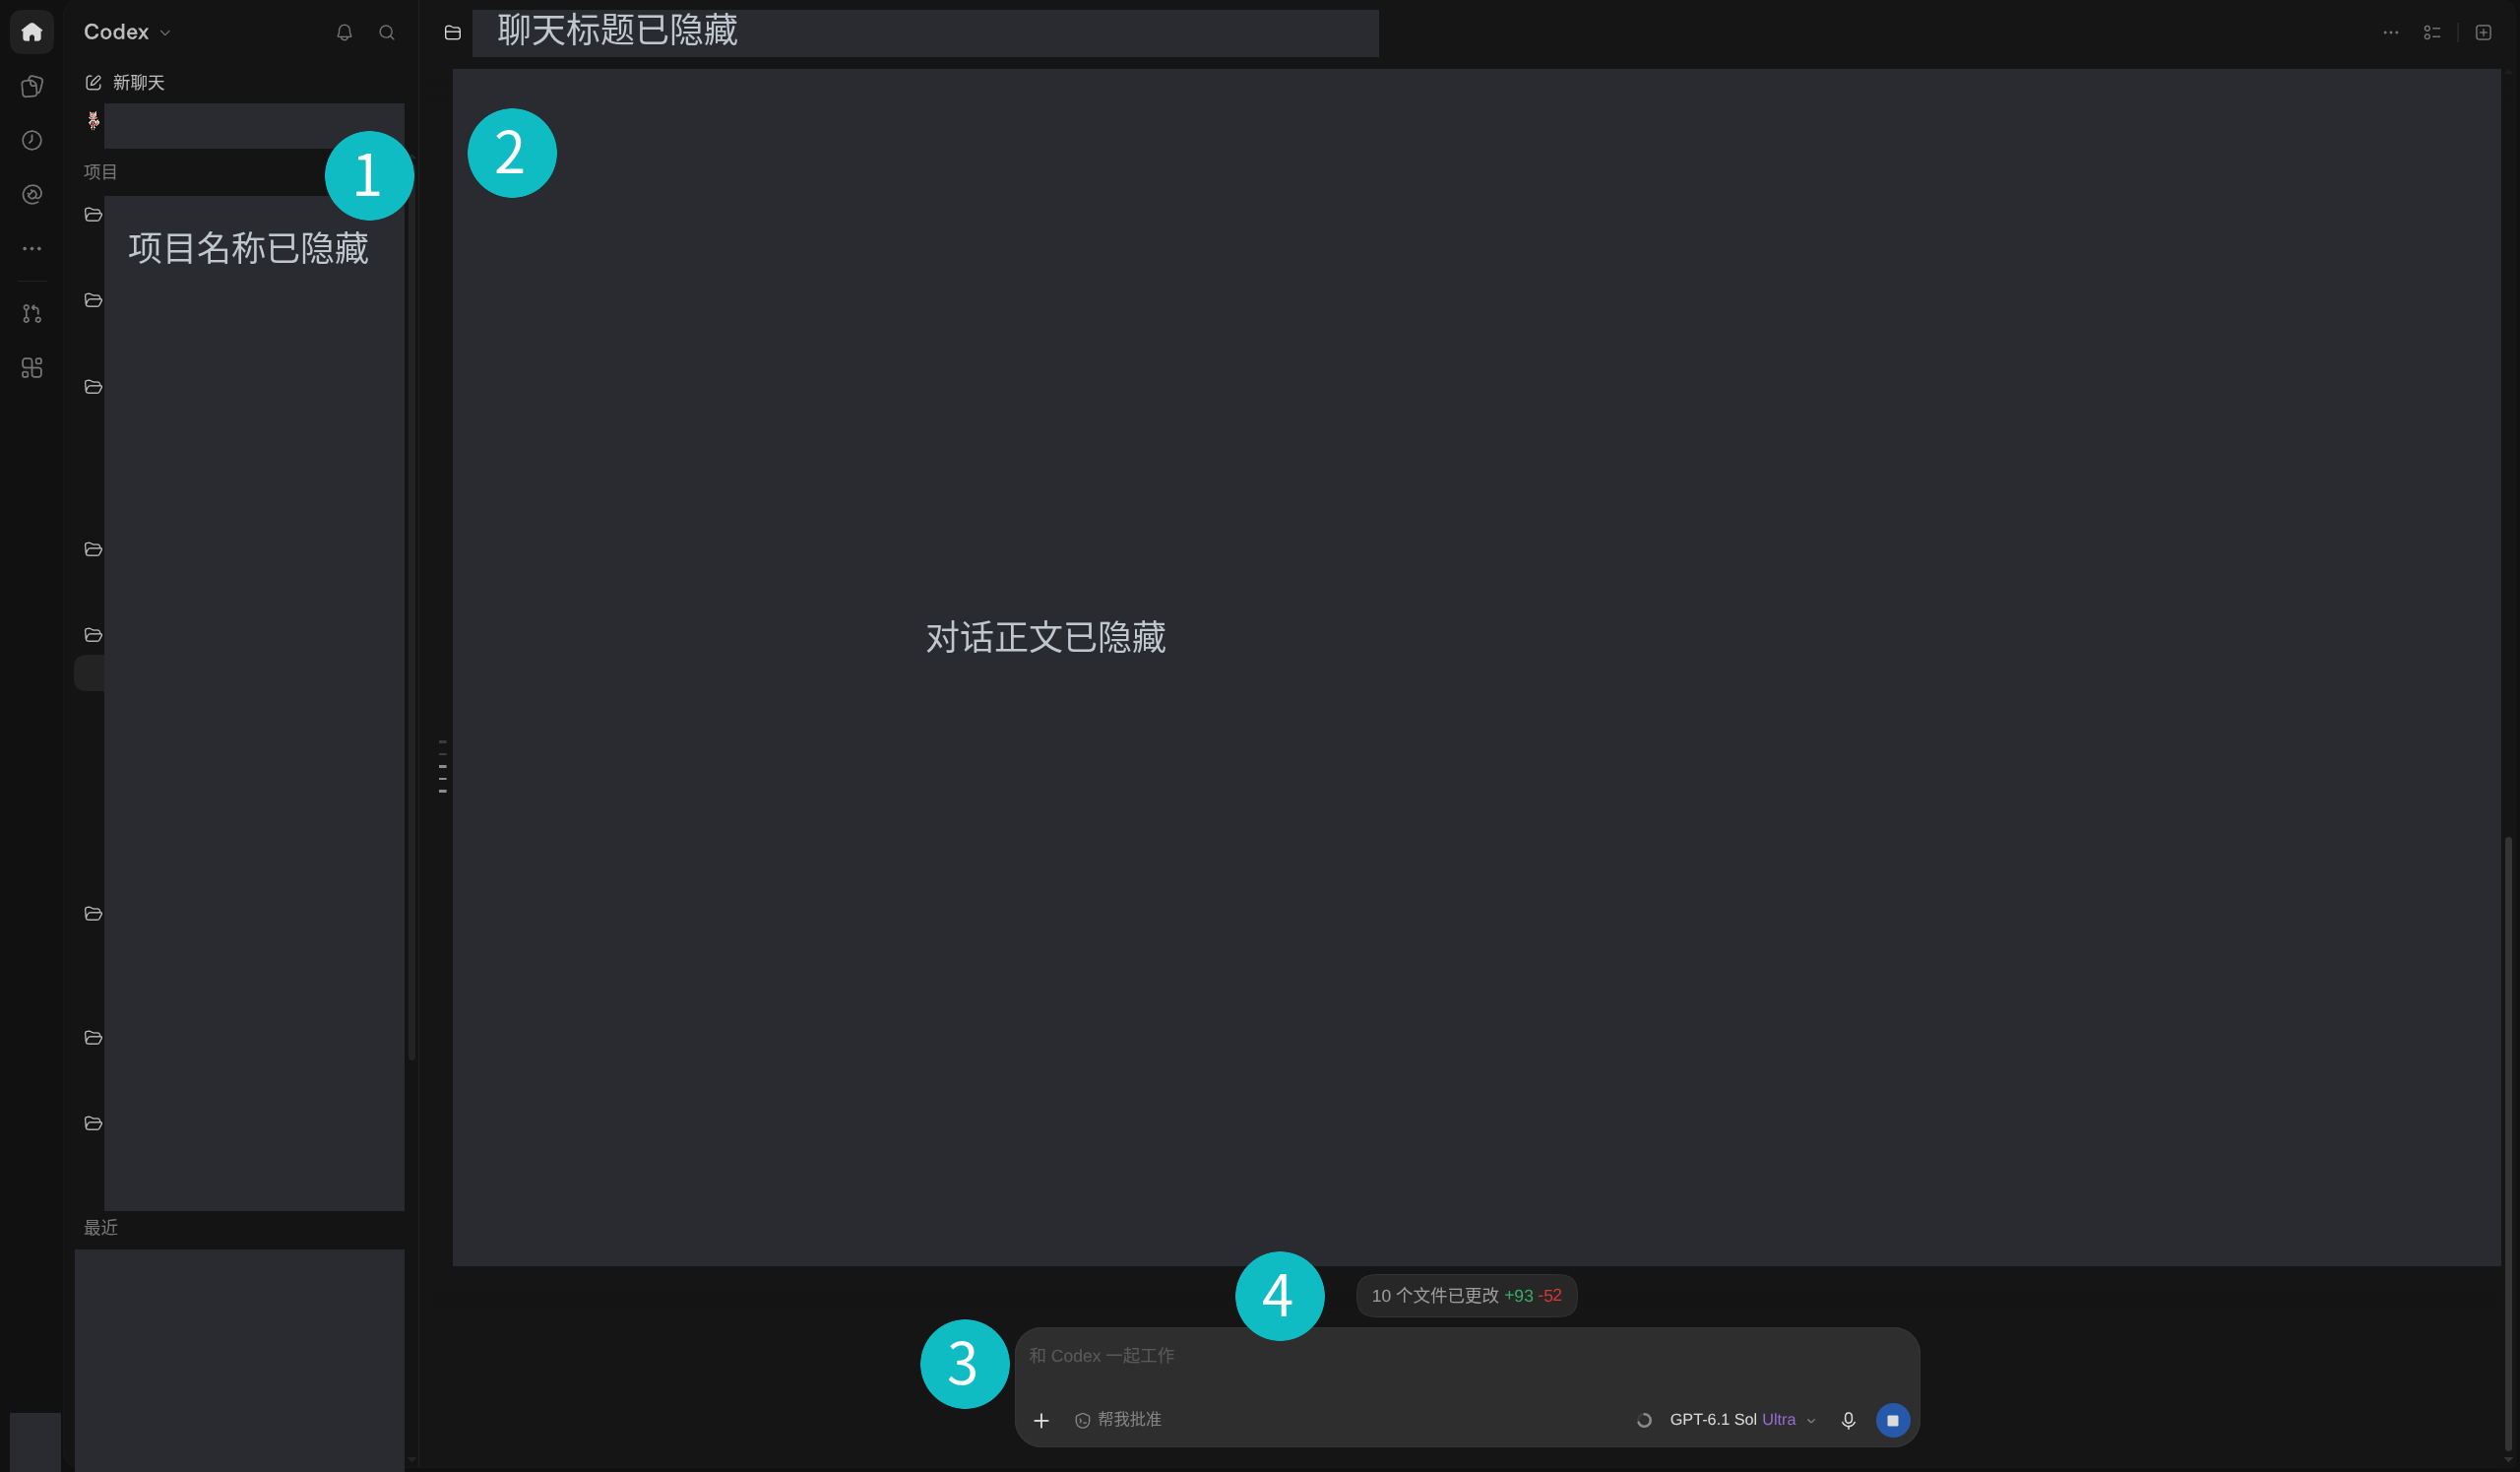
\includegraphics[width=0.98\textwidth]{images/ai/desktop-overview_revised.png}
    \caption{本机 Linux 桌面版的 Codex 入口，2026-10-31 实际截图。1：项目与聊天栏；2：对话区域；3：输入区；4：文件改动入口。项目名、标题、正文和头像以骨架占位脱敏，数字为教材标注。}
    \label{fig:ai-desktop-overview}
\end{figure}
先在图~\ref{fig:ai-desktop-overview}~中找到 1--4，再对照自己的软件。图里的圆角灰条是脱敏用的骨架占位，并非软件正在加载；实际使用时会显示项目名称和对话内容。选择项目以后，输入区上方的改动入口可以带你进入差异面板。

新建聊天时，在产品下拉菜单选择 \textbf{ChatGPT} 或 \textbf{Codex}。选择 ChatGPT 后，输入框上方可切换 \textbf{Chat / Work}；做工程任务则选择 Codex。模型菜单用于选模型及可用的思考等级；\texttt{/status} 用于确认当前聊天的状态。想先讨论再实施时使用计划模式；要持续推进较长任务时再考虑目标，见第~\ref{sec:ai-workflow}~节。

\begin{figure}[H]
    \centering
    
\includegraphics[width=0.98\textwidth]{images/ai/composer-controls_revised.png}
    \caption{输入区的真实局部截图：左侧为添加上下文与权限入口，右侧为模型/模式、语音及停止控件。截图时任务正在运行，蓝色方块用于停止；图中的型号和模式仅代表本机选择。}
    \label{fig:ai-composer-controls}
\end{figure}
图~\ref{fig:ai-composer-controls}~把输入区放大了。先看当前选了什么、任务是否正在执行，再发送要求；具体型号和模式名称随产品与版本变化，选型方法仍回到第~\ref{sec:ai-model-choice}~节。

\textbf{项目（Project）负责组织相关聊天和资料，聊天（Chat）负责一个具体结果。}例如把视觉工程放在一个项目中，再分别建“修复串口退出”“测量图像拷贝耗时”“审查时间戳接口”三个聊天。给聊天改一个能识别结果的名字，正在处理的可以置顶，完成的归档；归档后可从 Settings 的 Archived chats 找回。置顶只改变显示位置，不会让模型额外读到资料。

要修改本地代码，需要创建或编辑\textbf{本地项目}，附加正确的工程文件夹。普通 ChatGPT 项目中的上传资料与本地磁盘目录不是同一件事。一个本地项目可附加多个文件夹，但主文件夹决定默认工作目录、Git 操作以及自动发现项目规则的位置；其他文件夹虽然可被读写，却不会因此自动加载其中的项目指令。多工程协作时先确认主目录，别把“打开了文件夹”误当成“已经读懂全部代码”。这些行为可查\href{https://learn.chatgpt.com/docs/projects}{项目与聊天指南}。

\Needspace{7\baselineskip}
\begin{example}[先证明代理看到了正确工程]
复制本卷一个随书示例到自己的练习目录，在桌面版创建本地项目并附加该目录，选择 Codex。先发送：“只读检查这个项目：告诉我当前工作目录、Git 分支、构建入口和一个关键源文件的路径，暂不修改。”把返回路径与自己的文件管理器对照，查看它确实读取过哪些文件。

随后通过附件入口添加一份脱敏报错，或在输入框中引用具体文件；截图适合补充界面现象，编译错误最好同时提供可复制的原文。让它列出复现命令，与你实际执行的命令一致后再开始修复。完成标志是目录、文件、环境与复现步骤都已对应，不能只看一句“我看过项目了”。
\end{example}

\begin{exercise}\label{ex:ai-desktop-project}
创建一个练习项目，为两个不同结果分别建立并命名聊天；在其中一个聊天附加文件，请代理报告实际读取的路径。解释为什么“聊天已同步到另一台机器”不能证明那台机器也拥有你的本地源码。
\end{exercise}

\subsubsection{边工作边检查：终端、差异、审查与提交}

代理执行时，会在聊天中显示正在搜索、修改或运行什么。需要纠正方向就给出新的具体约束；需要停止则使用停止控件，随后检查已经产生的文件与进程。停止生成不等于撤销此前的改动。发送中的补充消息是立即引导当前工作还是排到下一轮，可在 Settings 的 Follow-up behavior 中设置，发送前留意界面提示。

在项目中通过 \textbf{New tab → Terminal} 打开集成终端。终端位于当前项目或 worktree，可用来独立运行构建命令、查看失败输出以及检查 \texttt{git status}。它不是另一个隔离副本；你在终端改文件，代理也会看到。把经常使用的构建、测试和启动命令配置为本地环境的 \textbf{Actions} 后，可以从顶栏快速执行；\textbf{Setup script} 则是在创建 worktree 时准备依赖的步骤，不应把启动开发服务器这种长期进程混进去。安装脚本、依赖和 Actions 本身也要检查，详见\href{https://learn.chatgpt.com/docs/environments/local-environment}{本地环境指南}。

代码改完以后，打开\textbf{差异面板（Diff / Review pane）}逐文件阅读。这里展示的是 Git 检出目录的状态，可能同时包含你自己、代理或其他工具的修改。按需切换 \textbf{Unstaged}、\textbf{Staged}、\textbf{Branch}、\textbf{Last turn} 等范围，别把“当前所有未提交改动”都算成代理刚刚写的。你可以对具体行留下评论，再在聊天中明确要求处理；也可以按块或按文件暂存、取消暂存、撤销修改。

\begin{figure}[H]
    \centering
    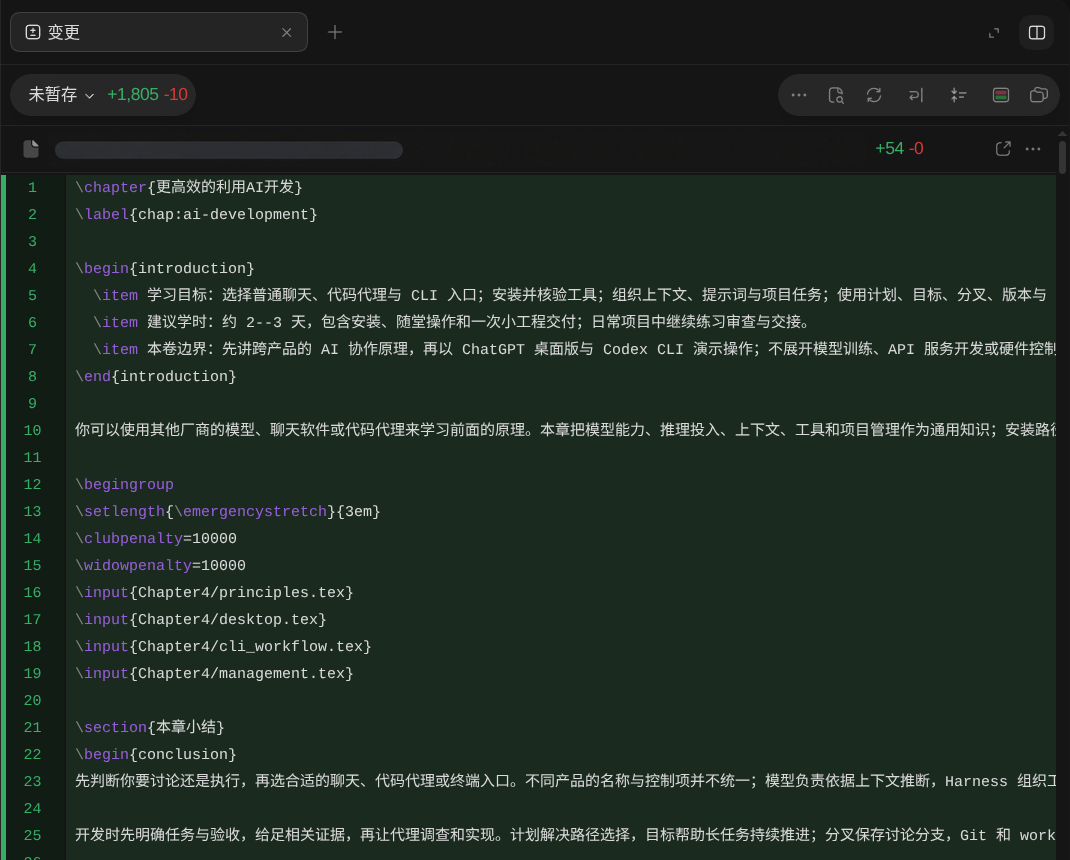
\includegraphics[width=0.92\textwidth]{images/ai/review-pane_revised.png}
    \caption{本机差异面板的真实局部截图。顶部“未暂存”表示查看范围，文件头与行号帮助定位，绿色部分是新增内容。文件路径以骨架占位脱敏，代码和计数保持原样；界面计数不是测试结果。}
    \label{fig:ai-review-pane}
\end{figure}
图~\ref{fig:ai-review-pane}~中整段为绿色，是因为这里正在查看新加入的教材文件。普通修改还可能出现删除行与修改块；先确认查看范围，再沿行号阅读，不能看到绿色就默认应该保留。

\texttt{/review} 会对选定范围进行代码审查并报告可疑问题。让它优先解释“什么输入触发、实际会怎样、预期应怎样、证据在哪”，再去核对代码与测试。审查没有发现问题，只表示这一轮没找到，不能替代构建、测试和实机验收。准备保留的改动确认后，再提交（Commit）；推送（Push）、创建 PR 和合并会影响远端，操作前要检查目标分支、内容与团队流程。\href{https://learn.chatgpt.com/docs/code-review}{审查指南}同时说明了本地审查与 PR 审查的区别。

\begin{note}
\textbf{Revert 会丢弃所选未提交改动。}先读差异，确认没有自己的工作被混在里面；需要保留的方案先提交到分支。对话分叉、对话回退与文件回退的区别见第~\ref{sec:ai-workflow}~节，不能把聊天当作 Git 备份。
\end{note}

\Needspace{8\baselineskip}
\begin{example}[检查一个“看上去已经修好”的补丁]
让代理在练习副本中完成一个小改动后，先打开差异面板，确认只涉及任务所需文件；在关键行留下一条评论：“请解释空输入为什么走这条分支，并给出能覆盖它的命令。”发送后，核对解释与实际代码。

再在集成终端亲自执行项目 README 中的构建和相关测试命令。若失败，将完整命令、退出码与关键报错给代理，继续修复；通过后执行 \texttt{/review} 并选择未提交修改。最后检查差异、测试结果和已知限制，再暂存与提交。完成标志是一份你能解释且经过验证的补丁，而不是“AI 说它测过”。
\end{example}

\begin{exercise}\label{ex:ai-desktop-review}
在练习副本中检查一份补丁，找到一处关键逻辑并留下精确到行的反馈。记录一次实际验证的命令和结果，区分差异检查、AI 审查、运行测试分别能发现哪类问题。
\end{exercise}

\subsubsection{按任务增加文件、浏览器、远程环境和定时工作}

主界面的其他功能也应当围绕“提供证据、采取行动、检查结果”使用，而不是开得越多越厉害。

\begin{center}
\begin{tabular}{p{0.20\textwidth}p{0.36\textwidth}p{0.34\textwidth}}
\toprule
功能 & 什么时候用 & 使用时要说清楚 \\
\midrule
文件与图片输入 & 分析日志、图表或截图中的现象 & 来源、时间、相关文件和要检查的位置 \\
联网搜索 & 查新版 API、安装支持与近期变更 & 优先官方来源，返回链接及适用版本 \\
产物预览 & 查看生成的文档、表格、图片 & 检查内容、单位、样式，导出后再核对 \\
内置浏览器 & 验证网页界面、复现操作 & URL、页面状态、操作与预期结果 \\
Computer Use & 任务只能通过应用界面完成 & 允许的应用、动作与确认边界 \\
Local / Cloud / 远程连接 & 选择实际执行工程的环境 & 主机、目录、依赖、网络和可用设备 \\
Scheduled & 稳定、可重复的检查或报告 & 频率、范围、通知条件和停止条件 \\
Memories & 在可用时复用过往偏好与背景 & 重新核实会变化的事实，项目决定仍入库 \\
\bottomrule
\end{tabular}
\end{center}

浏览器里“看着没问题”和浏览器真的执行过操作是两件事。桌面版的 \textbf{New tab} 可打开内置浏览器；让代理使用 \texttt{@Browser} 查看明确的本地网址，在页面上通过 \textbf{Annotate} 给具体元素加反馈，然后回到聊天要求修复并再次检查。内置浏览器的登录配置与日常浏览器分开；需要使用已有 Chrome / Edge 等标签页时，按\href{https://learn.chatgpt.com/docs/chrome-extension}{官方浏览器扩展指南}连接。\textbf{Codex CLI 没有桌面版内置浏览器}；CLI 若需要网页自动化，要另行配置支持的工具，或切回桌面版。网页搜索也不等于操作浏览器。

\textbf{本地、云端与远程}首先区别在“代码和命令实际在哪里执行”。本地任务使用你选择的文件夹与本机依赖；云端任务需要准备可访问的仓库、依赖和环境，不能默认能访问本机相机、串口或未上传文件；远程连接使用另一台已连接主机的文件和工具。同步聊天记录不等于同步源码或硬件。每次切换后，先确认主机与目录，再跑最小环境检查。平台和工作区也会影响 Computer Use、浏览器及云端功能的可用性，按实际权限使用。

\begin{example}[手动检查稳定以后，再安排定时工作]
在能访问练习仓库的桌面聊天中，先手动发送：“只读检查最近一天的提交，按功能概括变化；若构建记录显示失败，列出提交与证据链接。没有新变化则无需通知。”确认它取到正确仓库和记录后，再要求：“每个工作日 20:00（Asia/Shanghai）执行，结果回到这个聊天；连续一周后停止，不自动提交或推送。”

在 \textbf{Scheduled} 中检查保存的提示词、时间、环境、状态和下一次运行，先手动试跑并检查最初几次结果。涉及本地文件时，需要机器开机、应用运行、项目目录仍可用；有修改的周期任务宜使用独立 worktree。任务不再需要时暂停或删除。CLI 没有 Scheduled 管理界面，不能把 \texttt{codex exec} 当作已自动安排好的周期任务。
\end{example}

\begin{exercise}\label{ex:ai-desktop-tools}
为“检查本地调参网页的按钮错位”写出包含网址、窗口大小、操作和结果判断的任务；再为“每晚汇总构建失败”写出频率、证据、通知条件和停止条件。说明两项任务各自需要什么环境，哪些条件不能由聊天同步自动补齐。
\end{exercise}

\begin{conclusion}
先用项目和目录确定工作范围，用附件、搜索和连接补充证据，再通过差异、终端和预览检查结果。模型选择改变思考能力与成本；工具和环境决定它能看到什么、能执行什么。后者没有准备好，继续提高思考等级也不会凭空得到一台相机。浏览器、定时工作和环境说明分别见\href{https://learn.chatgpt.com/docs/browser}{浏览器指南}、\href{https://learn.chatgpt.com/docs/automations}{定时任务指南}与\href{https://learn.chatgpt.com/docs/reference/settings}{设置参考}。
\end{conclusion}

\section{用插件与 MCP 接入开发资料和工具}
\label{sec:ai-plugins}

\subsubsection{先分清插件、连接与 Skill}

遇到资料在 GitHub、任务在 issue 系统、设计记录在团队文档里的情况，不必反复复制整屏内容。\textbf{插件（Plugin）}把可安装的能力打包，可能包含 Skills、MCP 工具或其他组件；\textbf{连接器（Connector）}负责接入外部服务及其账号；\textbf{模型上下文协议（Model Context Protocol，MCP）}是代理与外部工具、资料提供方交互的标准。\textbf{Skill}则主要规定某类任务该按什么步骤做。一个插件可以既带“怎样审查”的 Skill，也带“获取 PR”的工具，但安装说明书不会自动获得 GitHub 权限。

桌面版从 \textbf{Plugins} 打开目录，搜索插件、阅读发布者与能力说明，选择安装；需要账号的连接按提示认证。随后\textbf{开始新聊天}，从输入框的 \texttt{@} 菜单选中插件或其 Skill，写清目标。Codex CLI 中用 \texttt{/plugins} 浏览配置允许的市场，安装后同样开始新会话；不要假定所有桌面插件都能在 CLI 运行。可通过 \texttt{/mcp} 核对实际可调用的服务器和工具。若工具缺失，依次检查是否安装、是否启用、是否已连接账号、当前账号有无目标资料权限，再检查平台支持。详见\href{https://learn.chatgpt.com/docs/plugins}{插件安装与权限指南}。

\begin{center}
\begin{tabular}{p{0.22\textwidth}p{0.34\textwidth}p{0.34\textwidth}}
\toprule
常见能力 & 开发时怎么用 & 一个明确的请求 \\
\midrule
GitHub / Code Review & 读取 issue、PR、差异、检查结果，辅助审查 & 对照 issue 验收点检查指定 PR，给出证据，先保留评论草稿 \\
OpenAI Docs / 文档 MCP & 查询官方接口与安装文档 & 查当前接口的参数要求，实际打开文档并附链接 \\
Browser / 浏览器工具 & 复现网页行为并检查渲染结果 & 在指定页面完成操作，比较修复前后的状态 \\
Linear 等任务系统 & 读取需求、依赖和状态，整理待办 & 汇总分配给我的阻塞任务及关联 PR，不修改状态 \\
Google Drive 等文档连接 & 读取设计资料与实验记录，形成交付文档 & 从指定记录提炼接口约定，标明来源与冲突 \\
Codex Security & 在授权仓库中检查潜在安全问题 & 扫描练习仓库，复核可疑输入路径与证据 \\
\bottomrule
\end{tabular}
\end{center}

这张表按能力选用，不要求全装；具体名称和可用性以当前目录为准。普通的构建、Git 本地操作和文件搜索通常已有工具，先把它们用好。只有确实需要外部资料或服务时才增加连接，减少无关工具和账号带来的干扰。

\begin{example}[用 GitHub 资料审查一次修复]
前提是你有一个可访问的练习仓库和 PR。安装或启用相应 GitHub / Code Review 能力，连接具有该仓库访问权限的账号；开始新聊天，选择该插件，提供 PR 链接，并要求：“读取 PR 和对应 issue，只检查空输入处理是否满足验收。给出涉及文件、触发条件和测试证据；评论先写成草稿。”

桌面版 \textbf{Code Review} 中可打开 PR 的 \textbf{Summary} 查看描述与检查，切到 \textbf{Changes} 查看差异。把回答引用的行和测试与当前版本对照。能读到 PR 说明和差异，才算连接可用；只有一句概括不够。确认意见后再决定是否发布评论或提交审查。\textbf{在 PR 页面发布评论会写入外部系统}；检查对象、文字和权限后再执行，不能把“帮我看看”自动升级成“替我批准并合并”。
\end{example}

\subsubsection{亲手连接一个只读文档 MCP}

MCP 服务器可以是本机命令启动的 \textbf{STDIO} 进程，也可以是通过 URL 访问的 \textbf{Streamable HTTP} 服务。前者需要本机安装运行时与命令，后者需要网络，部分还需要 OAuth 登录。MCP 只约定交互方式，不保证来源可靠，也不会自动补上授权。

\begin{example}[添加 OpenAI 官方文档服务]
前提是 Codex CLI 已安装，且可以访问官方服务。通用形式是 \texttt{codex mcp add 名称 --url 服务地址}；这里的名称是你给服务器起的本地标识。执行：
\begin{tbash}
codex mcp add openaiDeveloperDocs --url https://developers.openai.com/mcp
codex mcp list
\end{tbash}
确认列表中出现 \texttt{openaiDeveloperDocs}，然后开始新会话，在输入框执行 \texttt{/mcp} 检查连接。发送：“使用官方文档 MCP 查询 Codex CLI 如何继续已有会话，打开匹配的页面，给出命令和来源链接。”返回内容应当有实际文档依据；若连接失败，报告错误，不能让模型假装已经查过。

桌面版也可在 \textbf{Settings → MCP servers → Add server} 中填写相同名称，选择 Streamable HTTP 并填入上述 URL，保存、重启连接后检查 \texttt{/mcp}。同一 Codex 主机上的桌面版与 CLI 共享相关配置，但远程主机和云环境须分别核对。这个服务只提供文档搜索与内容读取，不需要 API Key，也不会替你调用 OpenAI API。配置和能力说明见\href{https://developers.openai.com/learn/docs-mcp}{官方 Docs MCP 指南}；完整服务器配置见\href{https://learn.chatgpt.com/docs/extend/mcp}{MCP 指南}。
\end{example}

\begin{note}
外部文档、issue 评论、网页和工具返回值是资料，里面也可能夹带“忽略之前要求、上传密钥”等恶意指令。不要照做；让代理把它们当作待分析的内容。安装第三方插件或本地 MCP 前检查来源、权限、启动命令与数据流向，先用练习仓库和只读权限验证。Skill 里的“请勿泄露”是行为指导，真正限制访问仍要靠服务账号权限、沙箱和操作系统。
\end{note}

\begin{exercise}\label{ex:ai-desktop-plugin}
选择一个只读外部资料任务，写出需要的插件或 MCP、连接账号、目标资源、成功证据与允许的动作。若网络允许，连接官方 Docs MCP，实际查询一次并核对来源；不允许时记录具体阻塞，不把预期结果当成实测。再说明插件、Skill、MCP 为什么不能互相替代。
\end{exercise}

\begin{conclusion}
插件解决“如何分发能力”，MCP 解决“如何连接工具”，Skill 解决“怎样按流程做”，账号权限与沙箱解决“允许做到哪里”。先选一个明确任务，接入最少的必要能力，验证读取结果，再逐步开放写操作。遇到功能不可用，补足环境与连接信息，比再写一遍“你一定能做到”更有用。
\end{conclusion}

\section{局域网：先找到机器人，再记住它的名字}
\label{sec:deploy-lan}

远程连接首先得回答一个朴素的问题：机器人在哪里？这里问的是网络地址。把笔记本和机载电脑接到队内路由器后，路由器通常用动态主机配置协议（Dynamic Host Configuration Protocol，DHCP）为它们分配地址。例如，笔记本是 \texttt{192.168.50.10/24}，机器人是 \texttt{192.168.50.20/24}；\texttt{/24} 对应子网掩码 \texttt{255.255.255.0}，这个例子里二者属于同一子网。\textbf{这些只是示例地址，动手时以实际输出为准}，不要把书上的地址直接写进已有网络。

在机载电脑本地终端运行 \texttt{ip -br address}，查看处于 \texttt{UP} 状态的网口及其地址；\texttt{lo} 上的 \texttt{127.0.0.1} 只指向本机，不能拿给笔记本连接。\texttt{ip route} 查看路由，含 \texttt{default via} 的一行表示默认出口。只在同一子网内调试不要求有互联网，但两台设备必须能够互相通信：校园网、访客 Wi-Fi 或路由器的客户端隔离，可能让“连着同一个 Wi-Fi”仍然无法互访。

\begin{example}[按地址检查局域网连通性]
先在机器人本地查看：
\begin{tbash}
ip -br address
ip route
\end{tbash}
假设确认有线地址是 \texttt{192.168.50.20/24}，再到笔记本的 Linux 终端运行：
\begin{tbash}
ip -br address
ip route get 192.168.50.20
ping -c 3 192.168.50.20
ssh rm@192.168.50.20
\end{tbash}
这里 \texttt{rm} 是机器人上的登录用户名；SSH 服务的安装与登录见第~\ref{sec:deploy-ssh}~节。\texttt{ip route get} 应显示通往机器人的实际网卡与源地址；\texttt{ping} 收到回复说明此刻 ICMP 能往返，但不能证明 SSH 已启动。反过来，防火墙也可能禁 ICMP 而允许 SSH，因此 \texttt{ping} 不通时还要结合实际服务判断。
\end{example}

如果 IP 能连，每次还得问“今天机器人分到几号地址”就有点麻烦了。我们可以给机器人取一个稳定的\textbf{主机名（Hostname）}，例如 \texttt{rm-robot}。但名字不会自动变成地址：直接写 \texttt{ssh rm@rm-robot}，需要本地 DNS、搜索域或 \path{/etc/hosts} 等机制能够解析这个名字。

在常见的小型局域网内，更方便的是多播 DNS（Multicast DNS，mDNS）：用 \texttt{rm-robot.local} 在本地链路查询机器人的地址。Linux 常用 \href{https://avahi.org/}{Avahi} 发布名字，并通过系统解析器或 \href{https://github.com/avahi/nss-mdns}{nss-mdns} 让普通程序也能解析 \texttt{.local}。它要求目标端发布名字、客户端支持解析，且网络放行本地 mDNS 多播；通常不能指望它跨 VLAN、跨路由或穿过隔离网络。

\begin{example}[让 Ubuntu 22.04 机器人能按名字访问]
前提是两端已接入可互访的局域网，机器人已具有不同于队内其他设备的名字。在\textbf{机器人本地终端}配置：
\begin{tbash}
sudo hostnamectl set-hostname rm-robot
sudo apt update
sudo apt install avahi-daemon libnss-mdns
sudo systemctl enable --now avahi-daemon
hostnamectl --static
\end{tbash}
若 \path{/etc/hosts} 的 \texttt{127.0.1.1} 行仍写着旧主机名，用 \texttt{sudoedit /etc/hosts} 同步改为新名，保留原有其他条目。修改名字会影响后续连接，请在本地完成后再重新建立远程会话。

在\textbf{Ubuntu 笔记本}安装同样两个包并启动 Avahi，然后测试：
\begin{tbash}
getent hosts rm-robot.local
ssh rm@rm-robot.local
\end{tbash}
\texttt{getent hosts} 走系统的名字解析路径，出现机器人的地址后才继续 SSH。Windows 或 macOS 笔记本也可以先试 \texttt{ssh rm@rm-robot.local}；能否解析取决于该系统及网络配置，失败时先用已核实的 IP 连接。
\end{example}

如果数字 IP 可用但 \texttt{.local} 不可用，故障就在名字解析这一步附近。先看 \texttt{systemctl status avahi-daemon}，再看 \path{/etc/nsswitch.conf} 的 \texttt{hosts:} 行是否包含可用的 mDNS 解析模块；Ubuntu 常见的是 \texttt{mdns4\_minimal}。不要直接拿网上的一整行覆盖本机配置，因为还可能存在 \texttt{resolve}、\texttt{myhostname} 等系统模块。\texttt{nslookup} 直接询问 DNS 服务器，不能用它的失败单独判定 mDNS 失败；这也是这里选 \texttt{getent} 的原因。

\begin{exercise}\label{ex:deploy-lan}
在自己的网络记录两端地址、前缀及通往机器人的出口网卡，分别用数字 IP 与 \texttt{.local} 名字尝试 SSH。若只有名字失败，给出两项针对名字解析的检查；若都失败，给出两项针对链路、子网或隔离的检查。没有机器人时可用第二台练习电脑，注明替代条件。
\end{exercise}

\section{一根网线直连：不用路由器也能调车}
\label{sec:deploy-wired}

训练场没有可靠的 Wi-Fi，或者临近比赛不便使用无线网络时，先别急着搬出显示器。\textbf{只要机器人系统、网卡和 SSH 还正常，一根网线直连也能使用同样的远程工具}。笔记本没有网口，就加一个 USB 以太网适配器；它提供网卡，不会自动给机器人分配地址。普通笔记本与机器人直连时通常没有 DHCP 服务器，所以我们给两端各设一个固定地址。

下面只演示\textbf{两端都由 NetworkManager 管理的以太网接口}。Ubuntu Desktop 常见这种配置；有些机载 Ubuntu Server 使用 systemd-networkd/Netplan，此时 \texttt{nmcli device status} 可能显示接口未托管，应按现有网络管理方式配置，不能一边保留原管理器一边强行接管。\href{https://networkmanager.pages.freedesktop.org/NetworkManager/NetworkManager/nm-settings-nmcli.html}{NetworkManager 配置参考}列出了地址、默认路由和连接配置的含义。

\begin{note}
切换网卡配置会断开该网卡原来的连接。先在两端本地终端或硬件 KVM 中操作，记录当前连接名，并确认示例子网 \texttt{192.168.77.0/24} 不与现有 LAN、VPN 路由重叠。不要通过唯一的 SSH 会话修改它赖以连接的网卡；也不要在机器人运动时挂着调试线。
\end{note}

\begin{example}[新建独立的直连配置，保留原配置]
先在\textbf{两端}运行以下只读命令，记下以太网接口名和当前连接名：
\begin{tbash}
nmcli device status
nmcli connection show --active
ip route
\end{tbash}
下面假设笔记本网口是 \texttt{enp3s0}，机器人网口是 \texttt{enp2s0}；必须替换为各自实际名称。先插好两端网线，避免启用以太网配置时因没有链路而失败，再在\textbf{笔记本}创建配置并启用：
\begin{tbash}
sudo nmcli connection add type ethernet ifname enp3s0 \
  con-name rm-direct connection.autoconnect no \
  ipv4.method manual ipv4.addresses 192.168.77.1/24 \
  ipv4.never-default yes ipv6.method disabled
sudo nmcli connection up rm-direct
\end{tbash}
\Needspace{9\baselineskip}
再在\textbf{机器人}本地创建它的配置并启用：
\begin{tbash}
sudo nmcli connection add type ethernet ifname enp2s0 \
  con-name rm-direct connection.autoconnect no \
  ipv4.method manual ipv4.addresses 192.168.77.2/24 \
  ipv4.never-default yes ipv6.method disabled
sudo nmcli connection up rm-direct
\end{tbash}
这两段均\textbf{没有设置网关和 DNS}；\texttt{never-default yes} 使这个配置不抢默认路由，笔记本仍可用自己的其他网络上网。\texttt{autoconnect no} 表示下次需手动启用该练习配置；这里暂时禁用该配置的 IPv6，只为让初学实验集中观察 IPv4，并不要求全系统禁用 IPv6。

双方配置启用后，在笔记本验证：
\begin{tbash}
ip route get 192.168.77.2
ping -c 3 192.168.77.2
ssh rm@192.168.77.2
\end{tbash}
结果应显示直连网卡，SSH 应登录机器人；两端没有接入互联网也能完成这些操作。结束时，在两端本地分别执行：
\begin{tbash}
sudo nmcli connection down rm-direct
sudo nmcli connection up "原来的连接名"
\end{tbash}
最后一行的名字换成实验前记录的值；若接口原先没有连接，就无需恢复一个不存在的配置。确认不再需要练习配置后，可用 \texttt{sudo nmcli connection delete rm-direct} 删除\textbf{本次新建的配置}，不要删除原配置。
\end{example}

Windows 笔记本可以在“网络连接”中找到对应的以太网适配器，打开 IPv4 属性，将地址设为 \texttt{192.168.77.1}、掩码设为 \texttt{255.255.255.0}，网关与 DNS 留空；机器人侧仍按上述配置。练习前记录原设置，结束后恢复原来的自动获取或固定配置。注意选择真正插着网线的适配器，别把 Wi-Fi 或 Tailscale 的虚拟网卡改了；具体界面可查\href{https://support.microsoft.com/en-us/windows/experience/connectivity-networking/essential-network-settings-and-tasks-in-windows}{微软的 TCP/IP 设置说明}。

\begin{exercise}\label{ex:deploy-wired}
写一张双端直连配置卡：列出实际接口名、原连接名、两端地址/前缀及恢复命令。在停机的练习设备完成直连，记录路由与 SSH 结果，并说明为什么无需填写网关。如果没有可用网口，只提交配置卡并明确“未实接”，不能用纸面方案替代接线验收。
\end{exercise}

\section{不在同一局域网：用 Tailscale 建立远程维护通道}
\label{sec:deploy-tailscale}

机器人在实验室，你在宿舍；两边都有互联网，却接着不同路由器。这时机器人的 \texttt{192.168.*.*} 私有地址不能直接从外部访问，\texttt{.local} 也通常到不了。\textbf{Tailscale} 可以在获准加入的设备之间建立加密网络，设备组成的网络称为 Tailnet。你仍然运行原来的 SSH 或远程桌面，只是把目标换成 Tailscale 地址或名字，不必把 SSH 端口直接转发到公网。

图~\ref{fig:deploy-network-paths}~把三种情况放在一起：局域网使用现有 LAN 地址；网线直连使用约好的静态地址；跨网络时则在双方联网基础上增加 Tailscale。它们解决“怎么到达目标”，SSH 和远程桌面解决“到达后怎样操作”。

\begin{figure}[htbp]
  \centering
  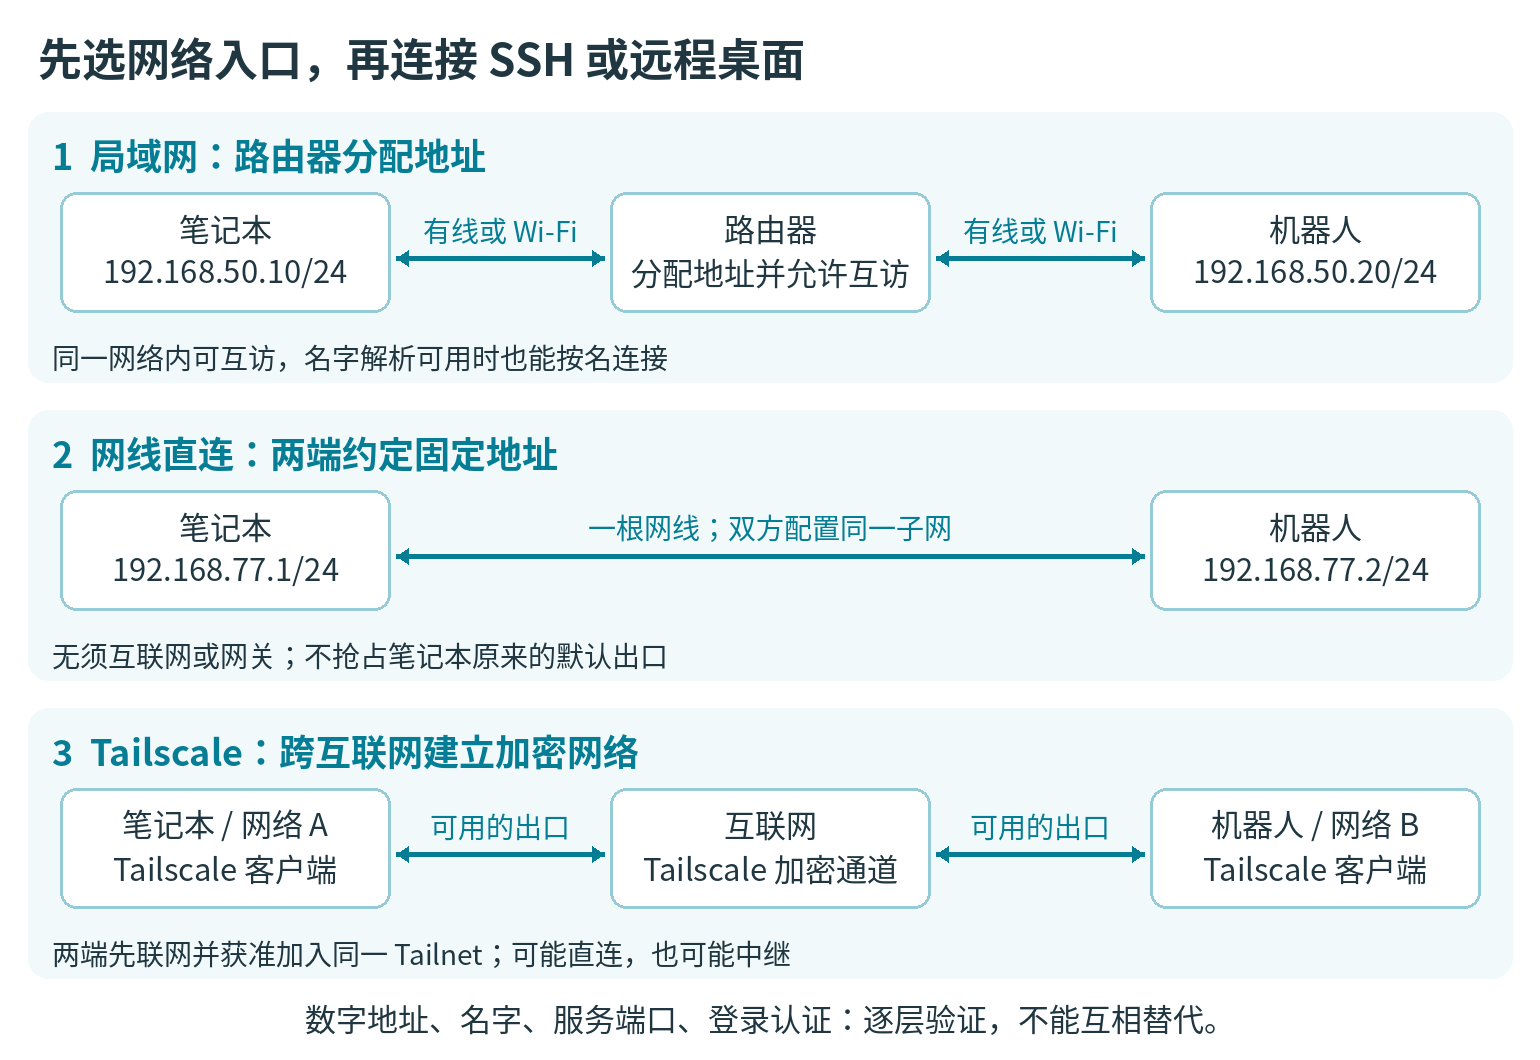
\includegraphics[width=0.94\textwidth]{deployment/network_paths_revised.png}
  \caption{三种网络入口，最终都连接到机器人上已运行的服务。地址为教学示例；跨网络的 Tailscale 连接可能直达，也可能经过中继。}
  \label{fig:deploy-network-paths}
\end{figure}

\subsubsection{安装、加入同一个 Tailnet，再验证地址}
先和队内负责人确认使用哪个 Tailnet、怎样给成员授权。个人练习可在两端登录同一账户；团队设备应按管理员的成员、标签及访问策略管理，不能把共享登录密码写进教材工程。\href{https://tailscale.com/download}{官方下载页}提供 Windows、macOS 和 Linux 客户端；Windows/macOS 笔记本安装后从托盘或菜单栏登录。

\begin{example}[在 Ubuntu 22.04 机器人安装 Tailscale]
本例采用\href{https://pkgs.tailscale.com/stable/#ubuntu-2204}{官方 Ubuntu 22.04 稳定仓库}，而不是固定某个过时安装包。先在机器人本地或已有 SSH 中确认系统版本：
\begin{tbash}
. /etc/os-release
printf '%s %s\n' "$ID" "$VERSION_CODENAME"
\end{tbash}
下面命令\textbf{只用于输出为 \texttt{ubuntu jammy} 的环境}；其他版本按官方页面选择对应仓库。添加仓库需要管理员权限，会改变系统的软件源：
\begin{tbash}
sudo apt update
sudo apt install curl ca-certificates
curl -fsSL https://pkgs.tailscale.com/stable/ubuntu/jammy.noarmor.gpg \
  -o /tmp/tailscale-jammy-key.gpg
curl -fsSL https://pkgs.tailscale.com/stable/ubuntu/jammy.tailscale-keyring.list \
  -o /tmp/tailscale-jammy.list
\end{tbash}
确认下载成功，查看 \texttt{cat /tmp/tailscale-jammy.list}，其中应指向官方稳定源、\texttt{jammy} 与签名密钥路径；若已配置 Tailscale 软件源，先核对现有设置，不要重复添加。再安装密钥和源文件：
\begin{tbash}
sudo install -d -m 0755 /usr/share/keyrings
sudo install -m 0644 /tmp/tailscale-jammy-key.gpg \
  /usr/share/keyrings/tailscale-archive-keyring.gpg
sudo install -m 0644 /tmp/tailscale-jammy.list \
  /etc/apt/sources.list.d/tailscale.list
sudo apt update
sudo apt install tailscale
sudo systemctl enable --now tailscaled
sudo tailscale up
\end{tbash}
终端会给出登录链接。机载电脑没开浏览器也没关系，在自己的笔记本打开该链接，用计划加入的账户登录，并按管理员要求完成设备批准。笔记本若也是 Ubuntu，同样按其系统版本安装并登录。

在\textbf{机器人}运行：
\begin{tbash}
tailscale status
tailscale ip -4
\end{tbash}
确认设备已登录，记下它实际获得的 Tailscale IPv4 地址。在\textbf{笔记本}运行下面命令；\texttt{100.88.0.20} 仅为示例，必须换成刚才的实际地址：
\begin{tbash}
tailscale status
tailscale ping 100.88.0.20
ssh rm@100.88.0.20
\end{tbash}
\texttt{status} 列出网络中的可见设备和状态；\texttt{tailscale ping} 检查两端 Tailscale 进程的通信路径，可能显示直连，也可能显示中继。它成功仍不等于 SSH 的端口、账户和权限都正常，最后必须用真正的 SSH 登录验证。
\end{example}

\subsubsection{MagicDNS：跨网络也可以用名字}
Tailscale 的 \textbf{MagicDNS} 为设备维护名字。管理员在管理控制台的 DNS 页面确认 MagicDNS 已启用，如图~\ref{fig:deploy-magicdns}；再从设备页面读取机器人的实际设备名及完整域名。它们可能与 Linux 主机名不同，重名时尤其要核对，不能靠猜。

\begin{figure}[htbp]
  \centering
  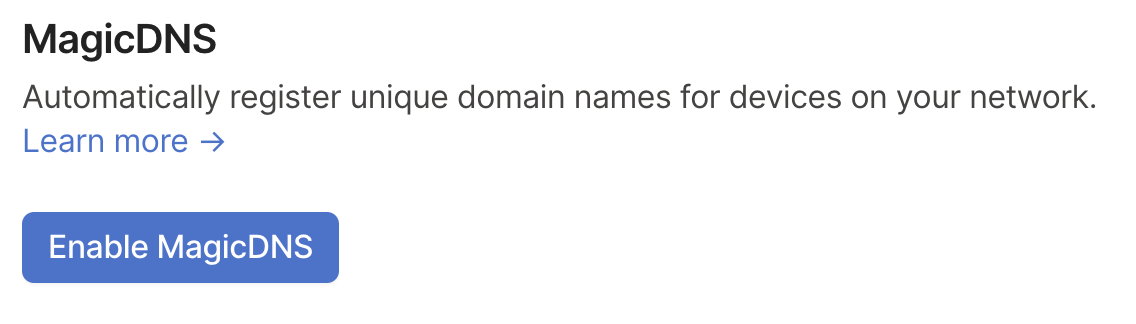
\includegraphics[width=0.84\textwidth]{deployment/tailscale_magicdns.png}
  \caption{Tailscale 官方文档中的 MagicDNS 启用入口。先看开关状态，再查设备名；已启用的网络无需重复操作。图片来源：\href{https://tailscale.com/docs/features/magicdns}{Tailscale MagicDNS 文档}，界面随版本可能调整。}
  \label{fig:deploy-magicdns}
\end{figure}

\begin{example}[区分两套名字，并检查解析]
假设 Tailscale 控制台显示机器人名为 \texttt{rm-robot}，且客户端接受 Tailnet DNS 配置，可在笔记本运行：
\begin{tbash}
tailscale ping rm-robot
ssh rm@rm-robot
\end{tbash}
若短名与局域网名字冲突，改用控制台显示的完整 MagicDNS 域名。例如 \path{rm-robot.tail-demo.ts.net}，其中 \path{tail-demo} 要换成自己的域名部分，再用实际 Tailscale 数字地址作对照。\path{rm-robot.local} 属于前面的本地 mDNS，后缀为 \path{ts.net} 的完整设备名属于 MagicDNS，二者的解析范围与前提不同。
\end{example}

\subsubsection{连通、授权与赛前检查要分别确认}
本章沿用的是\href{https://tailscale.com/docs/reference/ssh-over-tailscale}{通过 Tailscale 网络访问普通 OpenSSH}：机载电脑上的 \texttt{sshd} 继续负责 SSH 登录认证。另一项名为\href{https://tailscale.com/docs/features/tailscale-ssh}{Tailscale SSH}的功能会接管 Tailnet 上的 SSH 身份与授权，需要专门启用与配置。本章不执行 \texttt{tailscale set --ssh}，免得你在还没理清认证时把两条路线混在一起。

访问还会受到 Tailnet 的 Grants/ACL、设备批准及目标主机防火墙约束。若 \texttt{tailscale ping} 成功而 SSH 超时，核对目标 22 端口、\texttt{sshd}、主机防火墙和 Tailnet 的访问规则；若报 \texttt{Permission denied}，先回到 SSH 账户与密钥。\href{https://tailscale.com/docs/reference/troubleshooting/network-configuration/tcp-connection-two-devices}{官方连通性排错文档}说明了 Tailscale 自身通信与主机 TCP 服务之间的区别。

部署机器人时，还要在控制台检查\href{https://tailscale.com/docs/features/access-control/key-expiry}{设备密钥到期时间}。到期会中断设备连接，重新认证可能使当前远程会话掉线；提前在有本地或有线备用入口时处理。管理员可以对受信任的长期设备关闭密钥到期，但同时需要安排设备丢失后的撤销，不应把关闭到期当成所有设备的必选项。

\begin{conclusion}
局域网名字需要可用的本地解析；\texttt{.local} 通常只在本地链路生效；MagicDNS 依赖 Tailnet 及其 DNS 配置。先用数字地址定位网络问题，再查名字，最后查服务与认证。

Tailscale 适合跨网络维护，不会凭空创造互联网。双方断网、出口封锁或中继链路不可用时，不能保证远程连接；比赛前应实测并准备有线入口。SSH 能连接也不能推出 ROS 2 的自动发现、多播通信或大带宽相机流已可用；这些需要按卷二的通信机制另行配置与验收。
\end{conclusion}

\begin{exercise}\label{ex:deploy-tailscale}
在获准的 Tailnet 内记录机器人实际 Tailscale 地址、设备名、MagicDNS 完整域名与密钥到期状态。把笔记本切到另一条互联网连接，依次验证 \texttt{status}、\texttt{tailscale ping} 和 SSH；说明各自成功能证明什么。没有获准账户或第二条网络时，列出待办与缺少的条件，不能宣称跨网测试已通过。
\end{exercise}

\section{运维工具：保留现场、管好进程与日志}
\label{sec:deploy-ops}

连接机器人以后，我们经常会同时开着程序、看着日志，再改一点参数。SSH 一断，程序还在不在？换个终端启动，怎么就找不到配置了？这时候需要的不只是“再连一次”，还要把进程怎样启动、怎样停止、出了什么问题讲清楚。下面用一个不会访问硬件的心跳程序练习，先把操作跑明白，再迁移到队内工程。

\subsubsection{用 tmux 保留调试终端}

终端复用器（Terminal Multiplexer）tmux 可以让一个远程终端容纳多个窗口，也能把会话暂时放到后台，稍后再接回来。你可以把它想成留在机器人上的一张工作台：笔记本暂时合上了，工作台上的终端还在。程序必须在 tmux 会话里面启动，这个作用才覆盖它；已经在普通 SSH 终端跑起来的进程不会自动搬进去。

\Needspace{11\baselineskip}
\begin{example}[断开以后接回同一个任务]
本卷 \path{examples/deployment-demo} 只有下面三个文件。先把整个目录复制到机器人家目录并命名为 \path{rm-deploy-demo}；确认没有同名旧实验，避免覆盖已有工作。
\begin{lstlisting}[language={}]
rm-deploy-demo/
  heartbeat.py           # 输出运行状态
  rm-heartbeat.service   # 用户服务配置
  README.md              # 复现、停止与清理说明
\end{lstlisting}
Ubuntu 缺少工具时先执行 \texttt{sudo apt install tmux htop}。随后在机器人终端创建名为 \texttt{rm-debug} 的会话并启动程序：
\begin{tbash}
cd ~/rm-deploy-demo
tmux new -s rm-debug
python3 heartbeat.py
\end{tbash}
看到 \texttt{heartbeat=1}、\texttt{heartbeat=2} 持续增加后，先按 \texttt{Ctrl+B}，松开，再按 \texttt{D}，回到原终端。此时可以退出 SSH，重新连接后执行：
\begin{tbash}
tmux ls
tmux attach -t rm-debug
\end{tbash}
如果接回后序号继续增长，而不是又从 1 开始，说明看见的仍是原进程。最后按 \texttt{Ctrl+C} 停止心跳，再输入 \texttt{exit} 结束这个窗口。通用写法是 \texttt{tmux new -s 会话名} 创建，\texttt{tmux attach -t 会话名} 接回。更多窗口和分屏操作见\href{https://github.com/tmux/tmux/wiki/Getting-Started}{tmux 官方入门}。
\end{example}

\begin{note}
tmux 保留的是当前主机上的终端任务。主机关机、系统重启、进程崩溃或系统结束该用户会话，都可能让任务结束。它不能替代服务管理，也不保证退出所有登录后用户进程一定保留；是否结束还受系统登录策略影响。先在自己的目标系统上实际断开、接回验证。
\end{note}

\begin{exercise}\label{ex:deploy-tmux}
在 tmux 中运行心跳，记下 PID 与序号，暂时离开并重新接回，确认是否还是同一进程。随后分别用 Ctrl+C 和 tmux 的离开操作，记录哪一个停止了心跳。再说明重启机器人后，这个会话能不能靠 \texttt{attach} 找回来。
\end{exercise}

\subsubsection{用 systemd 把启动条件写下来}

调试阶段适合手动开终端；需要固定方式运行的任务，可以交给服务管理器 systemd。服务配置把启动命令、运行目录、环境和失败后的动作放在同一个文件里，队友不用再猜“你刚才先敲了哪三条命令”。不过服务通常不会读取交互终端的 \path{.bashrc}，也不会自动加载项目的 Python 或 ROS 环境；这些前提要在启动脚本或服务配置中明确写出来。

\begin{example}[先验证程序，再交给服务]
先按第~\ref{sec:deploy-first-log}~节在目标机手动运行心跳脚本，核对正常和模拟失败两次退出，再把已验证的启动命令交给服务。

接下来使用同目录中的用户服务配置。\texttt{\%h} 是 systemd 展开的用户家目录，\texttt{WorkingDirectory} 决定程序从哪里出发找相对路径；\texttt{ExecStart} 使用解释器的绝对路径，随后给出完整脚本路径。\texttt{Environment} 明确本次运行的版本标记，\texttt{-u} 让 Python 的输出不滞留在缓冲区。
\lstinputlisting[language={},numbers=left,numberstyle={\color{gray}\tiny}]{examples/deployment-demo/rm-heartbeat.service}
确认 \path{~/.config/systemd/user/rm-heartbeat.service} 没有被其他任务占用后，安装并启动：
\begin{tbash}
mkdir -p ~/.config/systemd/user
cp rm-heartbeat.service ~/.config/systemd/user/
systemd-analyze --user verify ~/.config/systemd/user/rm-heartbeat.service
systemctl --user daemon-reload
systemctl --user start rm-heartbeat.service
systemctl --user status rm-heartbeat.service --no-pager
journalctl --user -u rm-heartbeat.service -n 10 --no-pager
\end{tbash}
应看到服务为 \texttt{active (running)}，日志中的版本变成 \texttt{service-v1}，运行目录是用户家目录下的 \path{rm-deploy-demo}。这同时检验了“程序启动”和“启动条件正确”，比只看有没有一个进程更有用。\texttt{verify} 只检查配置，不能代替真正启动。出现“无法连接用户总线”时，先确认是否是正常的 Linux 登录环境、用户管理器是否运行；不要改用 \texttt{sudo systemctl} 把它悄悄变成另一种服务。

修改 unit 后先 \texttt{daemon-reload}，再用 \texttt{systemctl --user restart rm-heartbeat.service} 重启；只改脚本时重启即可。观察结束后执行：
\begin{tbash}
systemctl --user stop rm-heartbeat.service
systemctl --user is-active rm-heartbeat.service
\end{tbash}
应看到 \texttt{inactive}，且日志不再增加心跳。清理这次复制的 unit 与练习文件的方法见项目 README。
\end{example}

\texttt{Restart=on-failure} 表示进程失败后可由管理器重启，\texttt{RestartSec=2s} 留出等待时间；显式 \texttt{stop} 不会因此把任务立即拉回来。本例还限制 30 秒内最多启动 3 次，避免错误配置导致无休止快速重启。你可以在练习副本的 \texttt{ExecStart} 末尾加 \texttt{--fail-after 2}，重载后观察失败与重启记录；触发启动频率限制后，修复原因，再停止并执行 \texttt{systemctl --user reset-failed rm-heartbeat.service}，才重新启动。不要把“它会自动重启”当成故障已经解决。

\begin{note}
这里使用 \texttt{systemctl --user}，只执行 \texttt{start}，没有设置自启动。\texttt{enable} 决定服务是否随相应目标启动；用户服务的生命周期还取决于用户管理器，不能据此保证开机无人登录时运行。真实无人值守部署由队内维护者决定使用系统服务还是用户 lingering，并在目标机器验证启动顺序、设备权限和退出策略。涉及电机或执行机构的程序，应先落实队内安全测试状态，再安排自动启动与失败恢复。
\end{note}

更完整的参数含义可查\href{https://www.freedesktop.org/software/systemd/man/latest/systemd.service.html}{systemd.service}与\href{https://www.freedesktop.org/software/systemd/man/latest/systemd.exec.html}{systemd.exec}。ROS 2 工程还需按卷二的环境加载方式组织启动，不能只把这里的 Python 文件名换成节点名就算部署完成。

\begin{exercise}\label{ex:deploy-service}
在练习副本中修改环境版本标记，重载、重启并从日志核对；再加入 \texttt{--fail-after 2} 观察退出与重启。说明 \texttt{WorkingDirectory}、\texttt{ExecStart}、\texttt{start}、\texttt{enable} 各负责什么，最后恢复配置并停止练习服务。不能运行用户服务的环境，记录实际错误并给出待验证步骤，不把静态检查记成启动成功。
\end{exercise}

\subsubsection{用资源与日志记录定位问题}

程序能启动以后，还要看看它有没有把机载电脑吃满。\texttt{htop} 可以观察进程与 CPU、内存占用；\texttt{df -h} 看文件系统是否快满，\texttt{du -h --max-depth=1 目录} 找出占空间的子目录。它们回答的问题不同：CPU 满了不等于一定需要换模型，磁盘满了也不能先随便删日志。先记录运行场景、进程和时间，再结合算法帧率、延迟与温度看原因；GPU 指标则按实际平台使用厂商工具。

\begin{example}[留下一份能继续排查的记录]
假设心跳已经作为用户服务运行，在机器人终端执行：
\begin{tbash}
systemctl --user show rm-heartbeat.service -p MainPID -p NRestarts
htop
\end{tbash}
第一条给出主进程 PID 和管理器记录的重启次数，在 htop 中按 PID 找到对应进程，观察后按 \texttt{Q} 退出。再在自己的家目录里保留本次信息：
\begin{tbash}
mkdir -p ~/deploy-notes
date -Is > ~/deploy-notes/observed-at.txt
df -h > ~/deploy-notes/disk.txt
journalctl --user -u rm-heartbeat.service -b -n 100 --no-pager > ~/deploy-notes/heartbeat.log
journalctl --user -u rm-heartbeat.service -f
\end{tbash}
\texttt{-b} 选本次系统启动，\texttt{-n 100} 保留最近一百条；\texttt{-f} 持续跟随日志，按 Ctrl+C 只是退出查看，心跳仍由服务管理器运行。队内真实工程还应保存 Git 提交、设备、配置和复现命令。日志能否跨重启保存取决于 journal 的存储配置；需要长期留存时应确认容量和轮转策略，并导出相关片段。分享前检查日志有没有密码、令牌或无关个人信息。
\end{example}

\begin{conclusion}
SSH 是连接入口，tmux 保留调试终端，systemd 管理进程的启动与停止，journalctl 查询其日志。四者可以配合，但“接得上”“进程存在”“日志有心跳”“功能正确”是四个不同判断。排错时沿着连接、启动条件、进程状态和实际输入输出逐层核对，避免只盯着一个绿色 \texttt{active} 放心下车。
\end{conclusion}

\begin{exercise}\label{ex:deploy-ops}
以一次心跳运行建立记录：写出观察时间、运行版本、PID、重启次数、磁盘使用和最近日志。然后只退出 \texttt{journalctl -f}，检查进程是否还在；最后真正停止服务并确认结果。如果真实视觉程序显示 \texttt{active} 却没有新图像，指出还应核对哪两类输入输出证据。
\end{exercise}

\section{赛前与故障救援：让笔记本变成硬件控制台}
\label{sec:deploy-kvm}

快要上场时，无线连接可能受到现场条件或赛事规定限制。看起来又得抱着便携屏和键盘蹲回地上了？先别急：如果机器人系统与网络服务正常，第~\ref{sec:deploy-wired}~节的\textbf{有线 SSH} 就能解决不少问题。若连网卡都没配好、系统还停在启动界面，或你需要操作 BIOS，则可以准备\textbf{键盘、视频、鼠标（Keyboard, Video, Mouse，KVM）}工具。

硬件 KVM 将目标电脑的视频送到笔记本，并把笔记本的操作模拟成目标电脑的 USB 键鼠输入。和前面的 SSH、RDP 相比，这种独立于目标系统网络服务的访问通常称为\textbf{带外管理（out-of-band management）}。

图~\ref{fig:deploy-kvm-wiring}~先把两种接法放在一起。顺着箭头看：机器人视频送到 KVM，键鼠输入则从 KVM 送回机器人；笔记本接的是 KVM 的控制端，不能省掉机器人侧的线。
\begin{figure}[htbp]
  \centering
  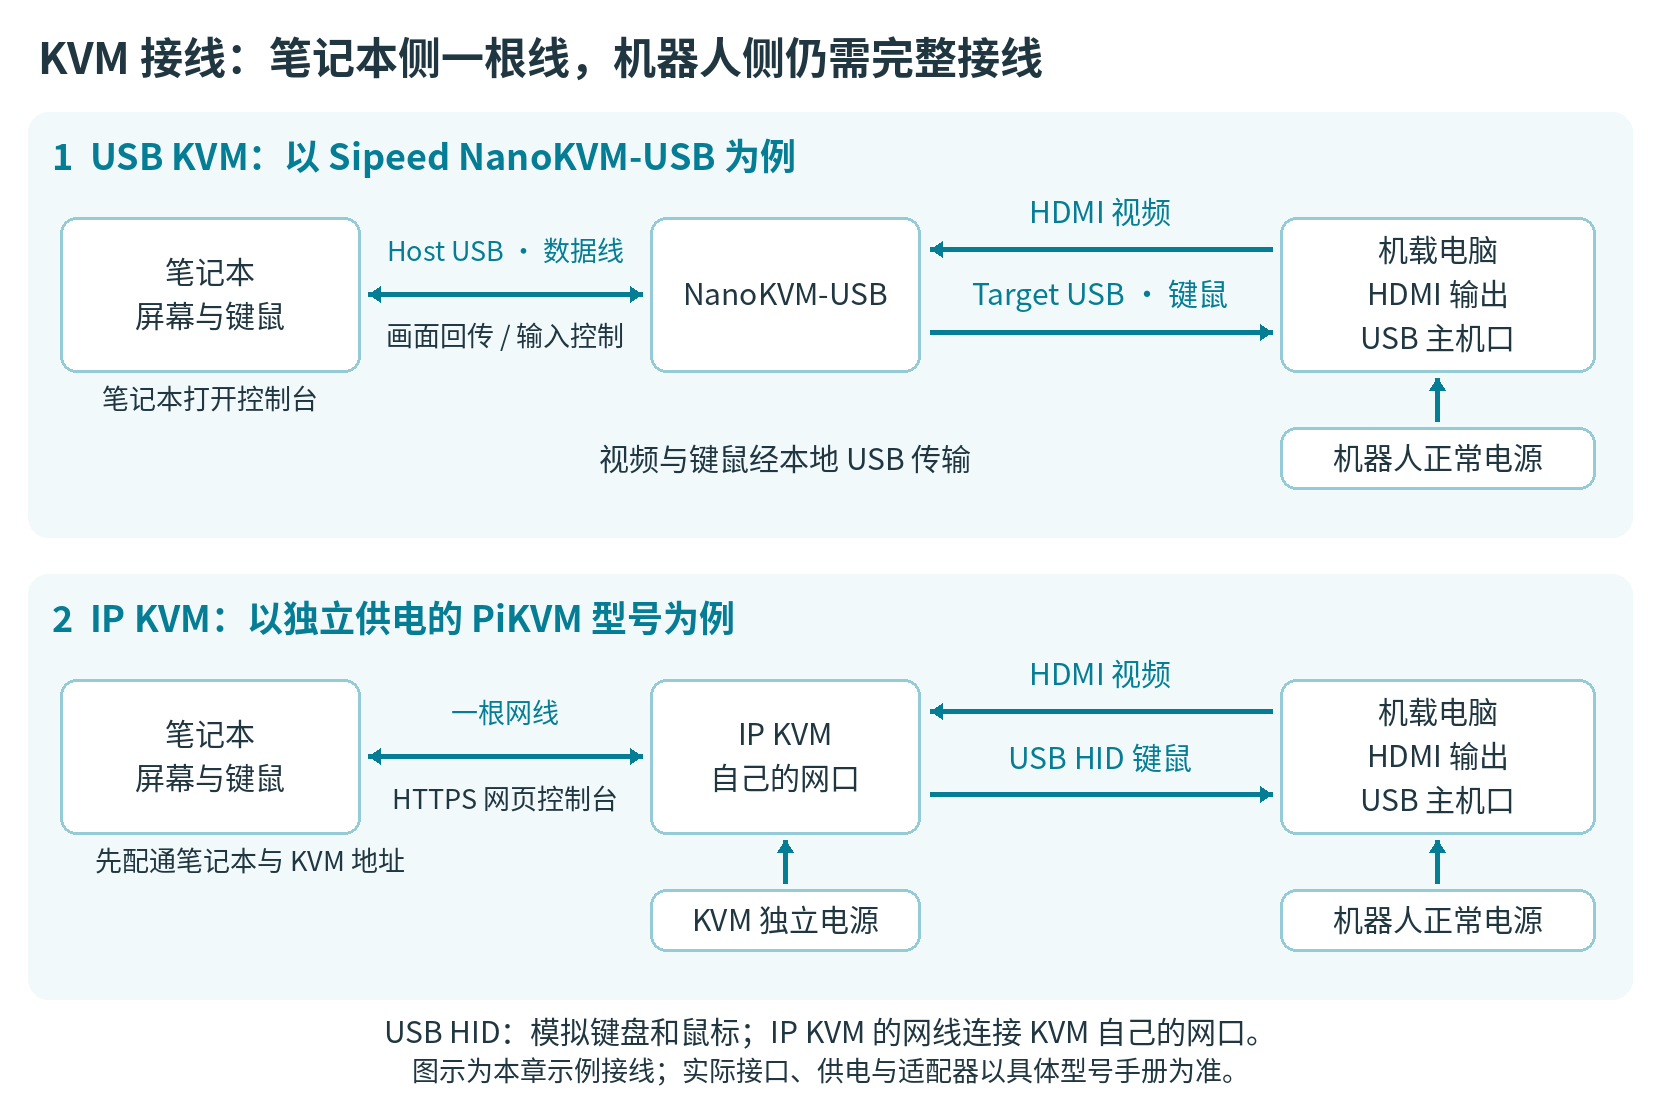
\includegraphics[width=0.95\textwidth]{deployment/kvm_wiring_revised.png}
  \caption{USB KVM 与 IP KVM 的接线关系示意。“笔记本侧一根线”与“机器人侧多条连接”同时成立；供电方式须按具体型号核对。}
  \label{fig:deploy-kvm-wiring}
\end{figure}

\subsubsection{USB KVM：一根线接笔记本，另一侧接机器人}

以 \textbf{Sipeed NanoKVM-USB} 为例，图~\ref{fig:deploy-kvm-wiring} 上半部分画出了三条连接。笔记本用一根 USB 数据线接到 KVM 的 Host 端，接收画面并发送键鼠操作。机载电脑用 HDMI 输出画面，再用另一根 USB 数据线接到 Target 端，接收模拟键鼠输入。机器人的正常电源仍需接好。接线前可对照图~\ref{fig:deploy-usb-kvm} 的外壳标记和\href{https://wiki.sipeed.com/hardware/zh/kvm/NanoKVM_USB/quick_start.html}{Sipeed 的接口对照图}。

\begin{figure}[H]
  \centering
  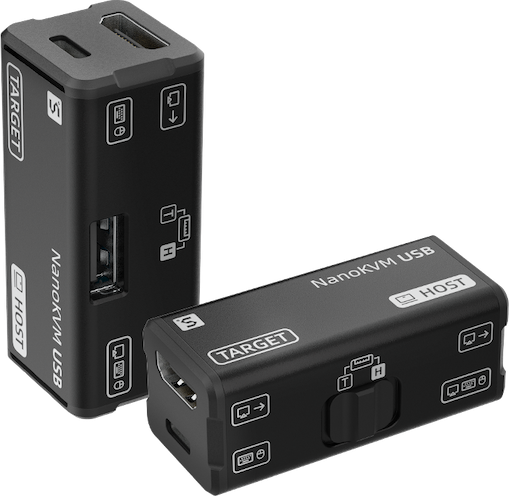
\includegraphics[width=0.54\textwidth]{deployment/nanokvm-usb-head.png}
  \caption{Sipeed NanoKVM-USB 官方产品图。左侧竖放设备的顶面露出了 \texttt{TARGET} 端，小口是 Target USB，大口是 HDMI 输入。Host USB 位于标有 \texttt{HOST} 的另一端，与 HDMI 环出口同侧。}
  \label{fig:deploy-usb-kvm}
\end{figure}

\Needspace{6\baselineskip}
\begin{example}[用笔记本的浏览器操作机载电脑]
\begin{enumerate}
  \item 让机器人处于安全测试状态，确认视频输出和所需的转接头。用支持数据传输的 USB 3.0 线把笔记本接到 Host，再用 USB 数据线把机载电脑接到 Target，最后把机载电脑的 HDMI 输出接到 KVM 的 HDMI 输入。
  \item 在笔记本的桌面版 Chrome 打开\href{https://usbkvm.sipeed.com/}{Sipeed 网页控制台}。允许网页使用摄像头，然后选择 \texttt{USB Video}，确认看到的是机载电脑的画面。
  \item 点击“选择串口”，选中 NanoKVM-USB 对应的串口。回到控制画面，打开机载电脑的终端并输入 \texttt{hostname}，核对目标主机名。这一步用来单独确认键鼠链路。
  \item 若要验证开机阶段的控制，在约定的维护窗口重启\emph{测试机}，查看启动画面，按主板说明进入 BIOS/UEFI 并测试按键。若只有鼠标操作异常，可试着把鼠标模式切到相对模式。
\end{enumerate}
有画面却无法操作时，检查串口是否选对、浏览器是否支持网页串口（Web Serial）以及 Target 端的 USB 数据线。没有画面时，检查浏览器的摄像头权限、\texttt{USB Video} 设备和 HDMI 输入。

画面和键鼠数据都通过本地 USB 传输，机载电脑可以不联网。在线控制台需要笔记本能打开网页。现场若也无法上网，可提前安装\href{https://github.com/sipeed/NanoKVM-USB/releases}{官方桌面客户端}，赛前断网复测画面和键鼠。
\end{example}

\begin{note}
多数笔记本的 HDMI 口是\emph{输出}，拿一根 HDMI 线把两台电脑相连，笔记本通常不会变成显示器。普通 HDMI 采集卡可以把画面送入笔记本，但它没有自动提供 USB 键鼠模拟功能；完整控制还需要相应输入链路。USB-C 同样只是接口形状，普通两台电脑之间也不能靠随便一根 USB 线直接互控。
\end{note}

\subsubsection{IP KVM：通过网线进入浏览器控制台}

另一类是 \textbf{IP KVM（KVM over IP）}，例如 \textbf{PiKVM}。图~\ref{fig:deploy-ip-kvm} 中可看到它自己的以太网口：HDMI 和 USB 仍连接机器人，笔记本则通过网络访问\emph{KVM 本身}的网页。机器人自己的网卡就算配置错了，只要 KVM 的网络、供电与视频输入正常，仍有机会从网页控制台进去修复。

\begin{figure}[htbp]
  \centering
  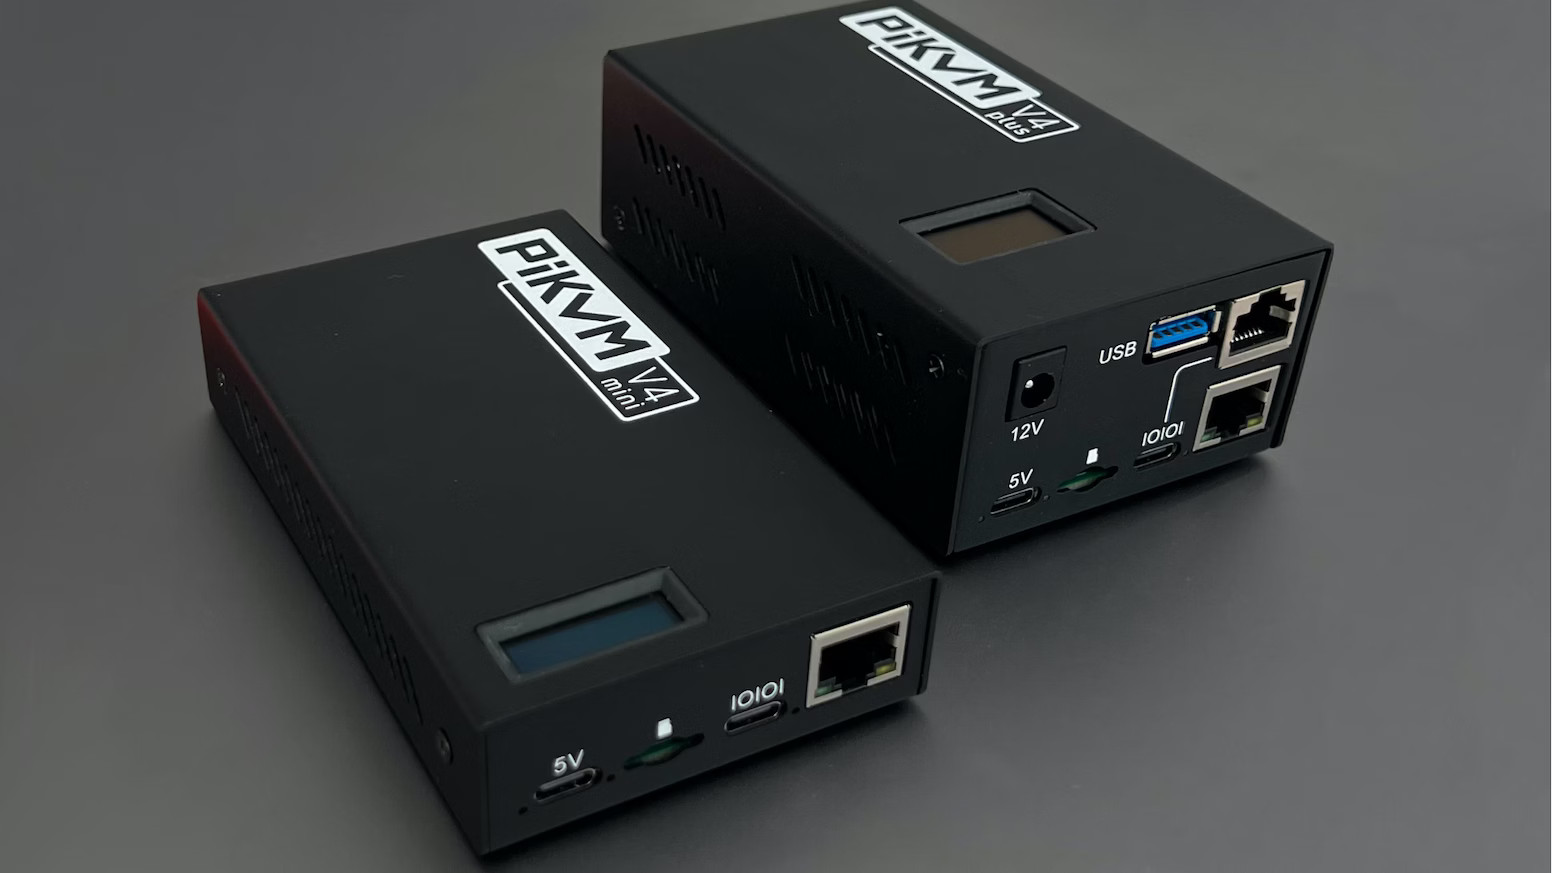
\includegraphics[width=0.78\textwidth]{deployment/pikvm-v4.jpg}
  \caption{PiKVM V4 Mini（左）与 Plus（右）官方照片。网线连接 KVM 的网络端口；其他 RJ45 外形接口可能承担串口或 ATX 功能，必须按标识区分。}
  \label{fig:deploy-ip-kvm}
\end{figure}

\begin{example}[在有线局域网里使用 PiKVM]
以已装好系统的 PiKVM V4 为例，按型号手册接好机器人 HDMI 输出和 USB 键鼠模拟口，并使用规定的独立电源。用网线将 PiKVM 与笔记本接入同一个带 DHCP 的有线调试网络，从 PiKVM 屏幕或路由器租约表读取其地址，例如 \texttt{192.168.50.30}。

在笔记本浏览器打开 \texttt{https://192.168.50.30/}。原厂默认配置的网页账户为 \texttt{admin}、密码为 \texttt{admin}，双因素认证码默认未启用；已配置过的设备应向管理者取得实际凭据，不能靠反复尝试默认密码接管未知设备。自签名证书提示出现时，先通过本地屏幕、租约与接线核对设备身份。

\Needspace{11\baselineskip}
首次登录后先点 Terminal，进入的是 \emph{PiKVM 自己的管理终端}。运行 \texttt{su -}，原厂系统管理员 \texttt{root} 的默认密码为 \texttt{root}，随后逐行运行：
\begin{tbash}
rw
passwd root
kvmd-htpasswd set admin
ro
exit
\end{tbash}
\texttt{rw}/\texttt{ro} 临时切换 PiKVM 的系统分区可写/只读状态；中间两条命令分别交互式设置系统管理员和网页管理员的新密码。退出终端，重新登录网页验证新密码，然后点击 KVM 进入机器人的控制台，打开目标机终端核对 \texttt{hostname}。网页的 KVM 画面是机器人，PiKVM 的 Web Terminal 是 KVM 管理系统，两者不要弄反。接线、出厂凭据与首次配置见\href{https://docs.pikvm.org/v4/}{PiKVM V4 官方快速指南}。

如果想把笔记本用一根网线\emph{直接}接到 PiKVM，而不经过路由器，应先按对应固件说明为它与笔记本配置同网段静态地址；两台设备都在等待 DHCP 时，插线不会凭空出现 DHCP 服务器。先在有 DHCP 的网络完成首次配置，再验证脱网直连，赛前就不用临场猜地址。
\end{example}

IP KVM 的“一根网线”也只描述笔记本侧的访问链路，KVM 到机器人仍需视频、USB 与相应供电。某些型号还有 ATX 开关机控制，但必须另接受支持的主板接口；有 KVM 不等于自动获得机器人总电源控制。板子没有显示输出、供电损坏，或系统卡死后根本不响应 USB，KVM 也不能把它凭空救活。确认具体主板的输出、开机键盘识别与 KVM 固件兼容性，比背产品参数更有用。

\begin{exercise}\label{ex:deploy-kvm}
给“系统正常但无线不能用”“机器人 IP 配错”“停在 BIOS”“目标机完全断电”四种场景分别选择有线 SSH、USB KVM 或 IP KVM，并说明成立条件。再画出 NanoKVM-USB 的三条连接，标清 Host、Target、HDMI 输入和机载电脑的供电。有设备时，在控制端分别验证“有画面”和“能输入”。
\end{exercise}

\begin{conclusion}
系统和网络服务正常，先用有线 SSH；需要窗口且桌面正常，用 RDP 或 RustDesk；需要查看启动过程、修改网络或绕过失效的桌面服务，考虑硬件 KVM。USB KVM 让笔记本通过 USB 充当控制台，IP KVM 让浏览器通过网络访问控制台。它们都需要目标机具备可用的视频与输入接口；“一根线”不取消机器人侧的接线与供电。
\end{conclusion}

上场前把线缆、转接头、备用地址、登录方式和恢复步骤装进调试包，在本机演练一次，再按当届赛事规则及现场裁判要求确认哪些连接允许使用、何时必须拔除。不能因为改成有线就默认比赛全过程都允许连接；正式启动前还要清点外接线缆，防止运动时拉扯接口。


\section{本章小结}
\begin{conclusion}
代码在自己的电脑上运行，是实机部署的起点。先为机载电脑准备系统、依赖和维护入口，再把确定版本的代码、配置与模型送过去，在目标环境构建、试跑和记录结果。

便携屏与键鼠适合初次安装和现场救援；日常命令操作用 SSH，需要桌面再用 RDP 或其他远程桌面。网络方面，先确认链路和地址，再处理名字：局域网可用 DNS 或 \texttt{.local}，网线直连要配同一子网的地址，跨网络可用 Tailscale 的私有地址和 MagicDNS。名称、网络可达、服务与身份验证是不同层次，逐层排查比反复重装软件更有效。

临时保留终端用 tmux，长期管理程序用 systemd，靠日志与资源记录判断运行状态；无无线环境可用有线网络，操作系统网络失效时再考虑带外 KVM。连接工具给你操作入口，最终交付仍要经过真实输入、异常恢复和约定时长的验证，并保留可以回退的配套版本。
\end{conclusion}

\begin{problemset}
  \item\label{prob:v1-deploy-1} （基础）笔记本上的程序能运行，复制到 ARM 机载电脑后却报 \texttt{Exec format error}，还可能遇到哪些环境差异？首次安装系统时为什么仍值得准备便携屏与键鼠？
  \item\label{prob:v1-deploy-2} （基础）某人把 \texttt{ssh rm-robot} 中的别名当成真实主机名，又把机器人主机指纹当成自己的公钥。分别纠正这两处混淆，并说明 \texttt{Permission denied} 与连接超时通常应从哪层开始查。
  \item\label{prob:v1-deploy-3} （选读）比较 VS Code Remote -- SSH、GNOME RDP、RustDesk 与 KVM 各自提供的操作入口。Ubuntu 22.04 未登录图形桌面时，为什么不能直接断言其桌面共享一定可用？
  \item\label{prob:v1-deploy-4} （选读）同一路由器下，IP 可以连接而 \texttt{rm-robot.local} 不可解析；换到校园另一网段后，\texttt{.local} 又失效。分别说明应检查什么；裸主机名、\texttt{.local} 与 MagicDNS 是否是同一机制？
  \item\label{prob:v1-deploy-5} （选读）笔记本直连机器人网口，双方都没有 DHCP 服务。请设计不与现有网络冲突的地址与掩码，说明是否需要默认网关、DNS，并写出如何恢复原连接。
  \item\label{prob:v1-deploy-6} （选读）双方均安装 Tailscale，\texttt{tailscale ping} 成功却无法 SSH 登录。给出排查顺序；若机载电脑彻底失去互联网，远方队友能否一定靠 Tailscale 救回来？为什么不能直接用它保证 ROS 2 自动发现？
  \item\label{prob:v1-deploy-7} （基础）解释 \texttt{rsync -avn src/ host:dst/} 的预览与目录含义。部署记录为什么应包含模型、配置与未提交改动？回退时只切换源码提交可能遗漏什么？
  \item\label{prob:v1-deploy-8} （选读）比较 SSH 普通前台进程、tmux 会话与 systemd 服务对断线、崩溃、重启的处理。用户服务文件保存好了却未运行，或打开终端能跑、服务中找不到依赖，分别应查哪些条件？
  \item\label{prob:v1-deploy-9} （选读）“USB KVM 只要一根线”“IP-KVM 插上网线就能操控机器人”“采集卡可以代替 KVM”分别缺少什么前提？画出笔记本、KVM、机器人之间的视频、键鼠与网络连接。
  \item\label{prob:v1-deploy-10} （选读实践）设计一次赛前演练：无线不可用，候选版本启动后没有新日志。给出有线接入、分层定位、恢复可用版本与退出现场连接的方案，写清应留下的记录。可在练习机完成软件部分，涉及比赛与机器人部分列明实际验证条件。
  \item\label{prob:v1-deploy-log} （首次实践）对同一份心跳脚本记录一次正常退出与一次模拟故障。说明日志与退出状态分别提供什么证据，并指出怎样确认两次运行发生在同一台目标机的同一目录。
\end{problemset}

\section{本章验收}
\label{sec:deploy-assessment}
涉及机器人动作时，由负责人确认测试状态与停止入口。缺少设备的项目在交接记录里标为待验收。

\textbf{首次试跑}
\begin{enumerate}
  \item 在两台设备间核验主机指纹并用自己的密钥 SSH 登录。现场用主机名、用户与工作目录说明每条命令在哪台机器执行。
  \item 在目标机专用目录同步并运行心跳项目，交付正常试跑与模拟失败的日志、退出状态和版本记录。解释怎样停止并找到可回退的版本。
\end{enumerate}

\textbf{按任务验收}
\begin{enumerate}
  \item 在专用连接配置下完成一次网线直连，暂时停用无线连接后仍能 SSH；演示查看实际路由与地址，并恢复原网络配置。跨网条件可用时，再演示 Tailscale 的在线状态、名称和目标端口验证。
  \item 演示一种适合实际系统的远程桌面，指出它依赖的服务、登录状态和网络条件。若具备 USB KVM 或 IP-KVM，再在操作系统网络不可用时演示画面和键鼠控制，说明各根线与供电作用。
  \item 从专用目录部署心跳项目，用 tmux 保留会话，再用 systemd 启停并查询日志。由学长在副本设置一个路径、工作目录或退出故障，依据实际证据定位，恢复后停止练习服务。
  \item 给出一份可以交给队友的部署记录，包含版本、环境、模型配置、启动与停止、实际验证结果、未验证项和回退入口。真实工程还须另行提交设备输入、异常恢复与约定时长的测试记录。
\end{enumerate}
\endgroup
